\documentclass[a4page,notitlepage]{article}
\usepackage{color,amsmath,graphicx,subcaption,geometry,mathtools}
\usepackage{cite}
\usepackage{mhchem}
\usepackage[dvipsnames]{xcolor}
\usepackage{tikz}
\usepackage{pgfplots}
\pgfplotsset{compat=1.12}
\usepackage{stackengine,ifthen}
\usetikzlibrary{arrows,positioning,calc,arrows.meta}
\tikzset{>=Latex}
\newcommand\influx{0.5}

\newenvironment{customlegend}[1][]{
  \begingroup
  \csname pgfplots@init@cleared@structures\endcsname
  \pgfplotsset{#1}
}{
  \csname pgfplots@createlegend\endcsname
  \endgroup
}

\def\addlegendimage{\csname pgfplots@addlegendimage\endcsname}
\setlength\abovecaptionskip{6pt}
\providecommand{\abs}[1]{\lvert#1\rvert}
\providecommand{\norm}[1]{\lVert#1\rVert}

\tikzset{>=latex}
%\tikzset{metaboliteStyle/.style={rectangle,draw}}
\tikzset{metaboliteStyle/.style={}}
\definecolor{cyan}{RGB}{100,181,205}
\definecolor{blue}{RGB}{76,114,176}
\definecolor{green}{RGB}{85,168,104}
\definecolor{magenta}{RGB}{129,114,178}
\definecolor{yellow}{RGB}{204,185,116}
\definecolor{red}{RGB}{196,78,82}

\colorlet{assimcol}{green}
\colorlet{sumcolor}{yellow}

\colorlet{inputcol}{green}
\colorlet{branchout}{red}
\colorlet{autocatacyc}{blue}
\colorlet{autocataby}{cyan}

\renewcommand\thesection{}
\renewcommand\thesubsection{}
\pdfpageattr{/Group <</S /Transparency /I true /CS /DeviceRGB>>} 
\title{Autocatalytic cycles stability constrains kinetic parameters of enzymes}
\author{Uri Barenholz, Dan Davidi, Yinon Bar-On, Elad Noor, Niv Antonovsky, Ron Milo}
\date{}

\begin{document}
\maketitle
\abstract{
    Autocatalytic cycles are an important part of metabolic networks.
    As the flux through autocatalytic cycles both depends on the concentration of intermediate metabolites and affects it, they present unique features and characteristics.
    We identify a few autocatalytic cycles in central carbon metabolism, some of which are generally not considered as such.
    Using the most simple form of autocatalytic cycle, we derive constraints of stability on kinetic parameters and show they are also relevant in the general case.
    The constraints we find are that, for stable fluxes through the cycle to occur, the autocatalytic reaction must have higher affinity and lower maximal flux than the reaction diverting metabolites out of the cycle for biomass generation.
    We discuss various extensions of the simple model including different kinetic functions and external fluxes into the cycle.
    We proceed to test these constraints based on experimental measurements in vivo and find these constraints to hold for functioning autocatalytic cycles for which data is available.
    This work thus serves as an approachable introduction to the analysis of autocatalytic metabolic cycles and as a demonstration of the insights one can get by such analysis on real networks.
}

\section{Introduction}
    Autocatalysis is generally defined as a setup in which one of the products of a chemical reaction is also a reactant in the same, or coupled reaction (see, for example, \cite{Steinfeld1999-iw}).
    A metabolic cycle is a set of reactions and corresponding metabolites that can be ordered in such a way that one of the products of each reaction is a substrate of the following reaction, with a product of the last reaction serving as a substrate for the first reaction.
    Metabolic cycles allow metabolites external to the cycle to serve as additional reactants or products of the reactions of the cycle.
    A metabolic cycle is autocatalytic if traversing the reactions that form the cycle increases the amount of the metabolites forming it.
    Surprisingly, autocatalytic cycles can be an essential building block of optimal metabolic networks \cite{Riehl2010-yh}.

    Autocatalytic cycles present specific metabolic control challenges as their inherent feed-back nature makes them susceptible to instabilities such as divergence or drainage of their intermediate metabolites \cite{Fell1999,Reznik2010-te}.
    Understanding the unique constraints that operating metabolic autocatalytic cycles impose is therefore essential for realizing limitations of existing metabolic networks, as well as for the introduction of modifications to them in synthetic biology metabolic engineering applications.

    The importance of autocatalytic cycles in metabolism is demonstrated by one of its most prominent examples, the Calvin-Benson-Bassham cycle (CBB) \cite{Benson1950-cl}.
    The CBB cycle, assimilating \ce{CO2} while converting 5-carbon compounds to 6-carbon compounds, serves as the main gateway for converting inorganic carbon to organic compounds in nature \cite{Raven2012-le}.
    We show that more autocatalytic cycles exist in central carbon metabolism, suggesting important biological insights can be gained by understanding the constraints underlying their stable operation.

    In this work we present the specific requirements autocatalytic cycles must meet in order to operate: (A) To be able to achieve at least one, non-zero, steady state of fluxes; 
    (B) To be stable in respect to fluctuations of metabolites or enzymes levels close to the steady state point(s).
    The mathematical tools we use are widely known and applicable in various fields (see, for example \cite{Strogatz2014-hp}).
    We identify the kinetic parameters of enzymes at metabolic branch points out of an autocatalytic cycle as the critical values that determine whether the cycle can function or not.
    Our analysis demonstrates the use of these results to gain insights about the operation, limitations, and various modifications available to metabolic autocatalytic cycles in vivo.

\section{Autocatalytic cycles play important roles in central carbon metabolism}
Different definitions exist for autocatalytic sets in the context of chemical reaction networks \cite{Hordijk2004-xe, Eigen2012-ti, Kun2008-xg}.
Here we define an autocatalytic cycle as a set of reactions and metabolites that form a cycle, and that, when the reactions are applied to the substrates at appropriate ratios, increase the amount of the intermediate metabolites.
Formally, a set of reactions and metabolites forms a cycle if:
\begin{itemize}
    \item Each metabolite of the set serves both as a substrate of at least one reaction of the set and as a product of at least one reaction of the set.
    \item At least one substrate of each reaction in the set, and one product of each reaction in the set are metabolites of the set.
\end{itemize}
A cycle is autocatalytic if the reactions of the cycle can be applied, each reaction at an appropriate, positive number of times, such that the resulting change in the amount of each of the metabolites forming the cycle is non-negative, with at least one metabolite of the cycle having a strictly positive change.
Three examples of autocatalytic cycles using central carbon metabolism are presented in figure \ref{fig:realautocatal}.

While less than a handful of autocatalytic cycles following this definition are widely known, a systematic search in central carbon metabolism yields several autocatalytic cycles that are not usually considered as such.
We find it useful to group the identified autocatalytic cycles in central carbon metabolism into four classes:
\begin{enumerate}
    \item The glyoxylate cycle within the TCA cycle, that can be used to produce two malate molecules from a single isocitrate molecule, assimilating acetyl-CoA, then converting the two malate molecules with extra acetyl-CoA into two isocitrate molecules \cite{Kornberg1966-lh}.
    \item Glycolysis based cycles using phosphoenolpyruvate (PEP) to transport sugar substrates using the phosphotransferase system (PTS), then converting the imported substrate into two PEP molecules.
    \item Various parts of the pentose-phosphate pathway (PP) assimilating imported sugars that are incorporated into central carbon metabolism as the intermediate metabolites: erythrose-4P, sedoheptulose-7P, ribose-5p or xylulose-5p to later produce these carbon compounds at higher stoichiometries.
    \item Cycles assimilating glycerone phosphate and using the Entner Doudoroff (ED) pathway \cite{Entner1952-xs}. They first use the fructose bisphosphate aldolase reaction in the reverse direction, producing fructose 1,6 bisphosphate from glyceraldehyde-3-phosphate, then convert the fructose back into two glyceraldehyde-3-phosphate.
\end{enumerate}

We note that the algorithm used in our systematic search is incomplete, meaning additional autocatalytic cycles may exist in central carbon metabolism.
Moreover, the algorithm is not optimized, resulting in an exponential increase in identified cycles when executed on the full metabolic network of \emph{E.coli} due to combinatorial combinations of elementary cycles to composite ones.
Further work will enable a more robust algorithm to identify additional autocatalytic cycles in the metabolic network.

The ubiquity of autocatalytic cycles in central carbon metabolism suggests that unique features of autocatalytic cycles, as derived below, may constrain and shape the kinetic parameters of a broad set of enzymes central to metabolism.

\begin{figure}[h!]
\resizebox{1\linewidth}{!}{
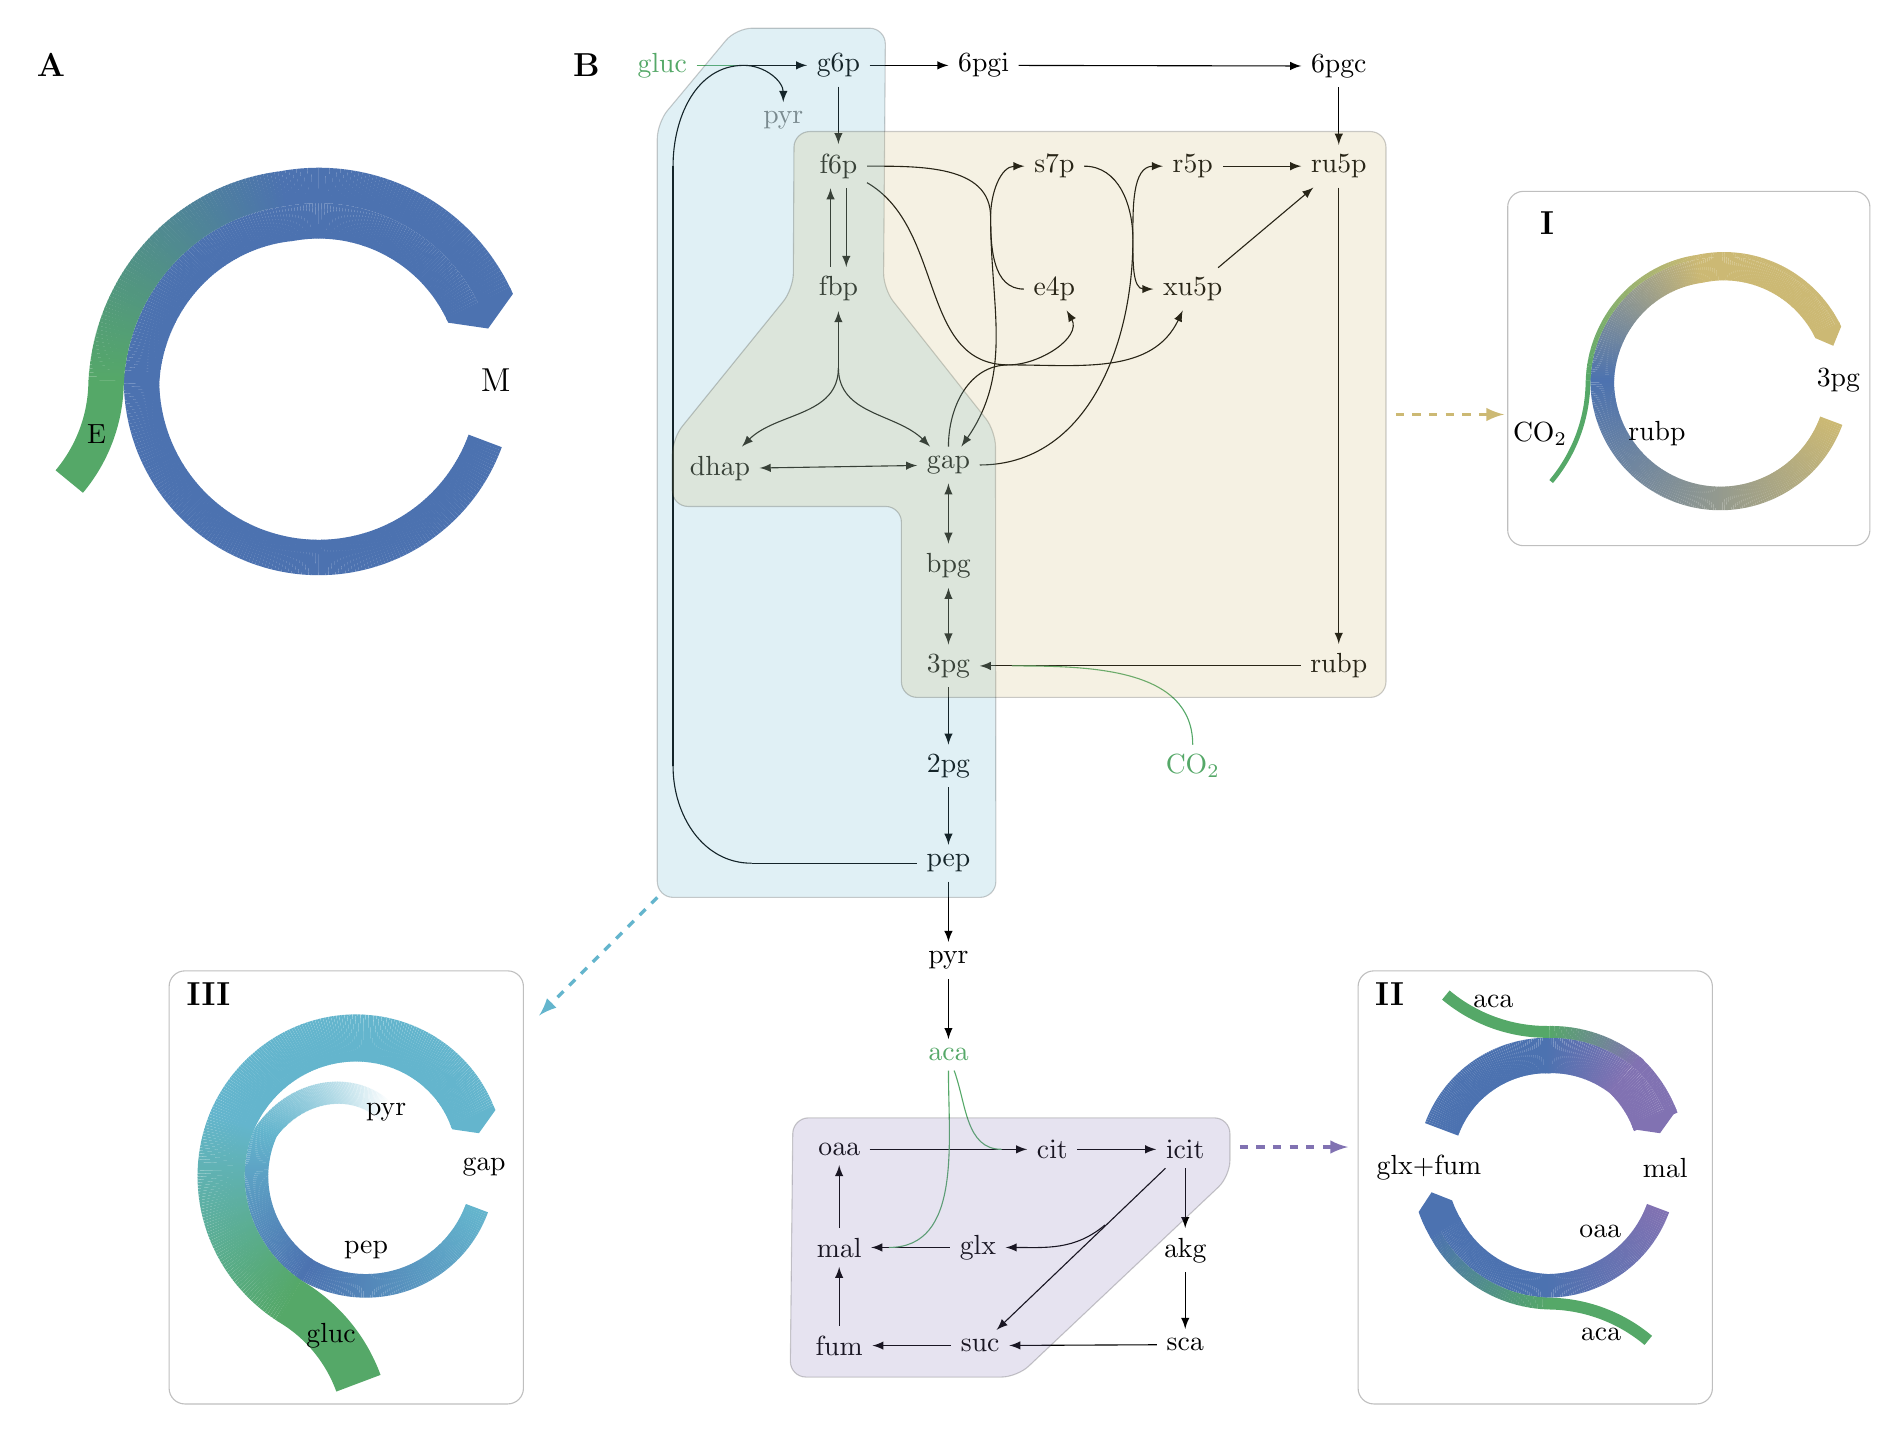
\begin{tikzpicture}
  \def\blendfrac{0.5}
  \def\deltaang{-155}
  \def\fromang{180}
  \def\inputang{-40}
  \def\protrude{7}
  \def\arcwidth{0.3cm}
  \def\highlightrad{0.2cm}
  \def\autocatalrad{1.5cm}
  \def\autocatalscale{1.5}
  \colorlet{ptsinit}{cyan}
  \colorlet{cbbinit}{yellow}
  \colorlet{glyinit}{magenta}

  \newcommand{\shadedarc}[7][\arcwidth]{%width,startang,stopang,startrad,stoprad,startcol,stopcol
    \pgfmathsetmacro\arcrange{#3-#2}
    \pgfmathsetmacro\radrange{#5-#4}
    \pgfmathsetmacro\progsign{\arcrange>0 ? 1 : -1}
    \foreach \i in {#2,...,\numexpr#3-1\relax} {
      \pgfmathsetmacro\fracprog{\i/\arcrange-#2/\arcrange}
      \pgfmathsetmacro\col{\fracprog*100}
      \draw[color={#6!\col!#7},line width=#1] (\i:#4+\radrange*\fracprog)
  arc[start angle=\i, end angle=\i+1.1*\progsign,radius=#4+\fracprog*\radrange];
    }
  }

  \newcommand{\coloredarc}[6][\arcwidth]{%width,startang,stopang,startrad,stoprad,startcol,stopcol
    \pgfmathsetmacro\arcrange{#3-#2}
    \pgfmathsetmacro\radrange{#5-#4}
    \pgfmathsetmacro\progsign{\arcrange>0 ? 1 : -1}
    \foreach \i in {#2,...,\numexpr#3-1\relax} {
      \pgfmathsetmacro\fracprog{\i/\arcrange-#2/\arcrange}
      \draw[color={#6},line width=#1] (\i:#4+\radrange*\fracprog)
        arc[start angle=\i, end angle=\i+1.1*\progsign,radius=#4+\fracprog*\radrange];
    }
  }


  \node[metaboliteStyle] (g6p) {g6p};

  %%%% upper pts
  \node[shape=coordinate,left=12mm of g6p.center] (ptsmid) {};
  \node[metaboliteStyle,assimcol,left=6mm of ptsmid] (gluc) {gluc};
  \node[metaboliteStyle,shift={(-7mm,-7mm)},gray] at (g6p.center) (pyr1) {pyr};
  \draw[assimcol] (gluc) -- (ptsmid);
  \draw[->] (ptsmid) [out=0,in=90] to (pyr1);

  \node[metaboliteStyle,below=of g6p.center] (f6p) {f6p};
  \node[metaboliteStyle,below=of f6p] (fbp) {fbp};
  \node[metaboliteStyle,shape=coordinate,below=of fbp.center](fbamid) {};
  \node[metaboliteStyle,below left=of fbamid.center] (dhap) {dhap};
  \node[metaboliteStyle,below right=of fbamid] (gap) {gap};
  \node[metaboliteStyle,below=of gap.center] (bpg) {bpg};
  \node[metaboliteStyle,below=of bpg.center] (3pg) {3pg};
  \node[metaboliteStyle,below=of 3pg.center] (2pg) {2pg};
  \node[metaboliteStyle,below=of 2pg.center] (pep) {pep};
  \node[metaboliteStyle,below=of pep.center] (pyr) {pyr};
  \node[metaboliteStyle,below=of pyr.center,assimcol] (aca) {aca};
  \node[shape=coordinate,below=of aca] (dummyglta) {};
  \node[metaboliteStyle,left=of dummyglta] (oaa) {oaa};
  \node[metaboliteStyle,right=of dummyglta] (cit) {cit};
  \node[metaboliteStyle,right=of cit] (icit) {icit};
  \node[metaboliteStyle,below=of icit.center] (akg) {akg};
  \node[metaboliteStyle,below=of akg.center] (sca) {sca};
  \node[metaboliteStyle,below=of oaa.center] (mal) {mal};
  \node[metaboliteStyle,below=of mal.center] (fum) {fum};
  \node[metaboliteStyle,right=of mal] (glx) {glx};
  \node[metaboliteStyle,right=of fum] (suc) {suc};
  \node[metaboliteStyle,right=of g6p] (6pgi) {6pgi};
  \node[metaboliteStyle,shape=coordinate,right=of f6p] (s7pspace) {};
  \node[metaboliteStyle,right=of s7pspace] (s7p) {s7p};
  \node[metaboliteStyle,right=of s7p] (r5p) {r5p};
  \node[metaboliteStyle,right=of r5p] (ru5p) {ru5p};
  \node[metaboliteStyle,above=of ru5p.center] (6pgc) {6pgc};
  \node[metaboliteStyle,] at (fbp.center -| s7p.center) (e4p) {e4p};
  \node[metaboliteStyle,] at(e4p.center -| r5p.center) (xu5p) {xu5p};
  \node[metaboliteStyle,] at(3pg.center -| ru5p.center) (rub) {rubp};
  \node[metaboliteStyle,assimcol] at(2pg -| xu5p.center) (co2) {\ce{CO2}};
  \draw[->] (g6p) -- (f6p);
  \draw[->] ([xshift=0.1cm]f6p.south) -- ([xshift=0.1cm]fbp.north);
  \draw[<-] ([xshift=-0.1cm]f6p.south) -- ([xshift=-0.1cm]fbp.north);
  \draw [<-] (fbp) [out=-90,in=90] to (fbamid);
  \draw [->] (fbamid) [out=-90,in=45] to (dhap);
  \draw [->] (fbamid) [out=-90,in=135] to (gap);
  \draw [<->] (dhap) -- (gap);
  \draw[<->] (gap) -- (bpg);
  \draw[<->] (bpg) -- (3pg);
  \draw[->] (3pg) -- (2pg);
  \draw[->] (2pg) -- (pep);
  \draw[->] (pep) -- (pyr);
  \draw[->] (pyr) -- (aca);
  \draw[->] (oaa) -- (cit) node [pos=0.9] (midglta) {};
  \draw [assimcol] (aca) [out=-70,in=180] to (midglta);
  \draw[->] (cit) -- (icit);
  \draw[->] (icit) -- (suc) node [pos=0.3] (midacea) {};
  \draw[->] (midacea) [out=220,in=0] to (glx);
  \draw[->] (icit) -- (akg);
  \draw[->] (akg) -- (sca);
  \draw[->] (sca) -- (suc);
  \draw[->] (suc) -- (fum);
  \draw[->] (fum) -- (mal);
  \draw[->] (glx) -- (mal) node [pos=0.9] (midaceb) {};
  \draw[->] (mal) -- (oaa);
  \draw[assimcol] (aca) [out=-90,in=0] to (midaceb);
  \draw[->] (g6p) -- (6pgi);
  \draw[->] (6pgi) -- (6pgc);
  \draw[->] (6pgc) -- (ru5p);
  \draw[<-] (ru5p) -- (xu5p);
  \draw[<-] (ru5p) -- (r5p);
  \path[] (r5p) -- (gap) coordinate [pos=0.2] (midtkt1) {};
  \draw[<-] (xu5p) [out=180,in=-90] to (midtkt1);
  \draw[] (midtkt1) [out=90,in=0] to (s7p);
  \draw[<-] (r5p) [out=180,in=90] to (midtkt1);
  \draw[] (midtkt1) [out=270,in=0] to (gap);
  \path[] (e4p) -- (gap) coordinate [pos=0.4] (midtkt2) {};
  \draw[<-] (e4p) [out=-60,in=0] to (midtkt2);
  \draw[] (midtkt2) [out=180,in=90] to (gap);
  \draw[<-] (xu5p) [out=245,in=0] to (midtkt2);
  \draw[] (midtkt2) [out=180,in=-30] to (f6p);
  \path[] (e4p) -- (s7pspace) coordinate [pos=0.5] (midtal) {};
  \draw[] (midtal) [out=90,in=0] to (f6p);
  \draw[<-] (s7p) [out=180,in=90] to (midtal);
  \draw[] (midtal) [out=-90,in=180] to (e4p);
  \draw[<-] (gap) [out=55,in=-90] to (midtal);
  %\node[metaboliteStyle,assimcol,shift={(-1.5,-0.8)}] at (pep.center) (gluc) {gluc};
  \node[shape=coordinate,left=2.5cm of pep.center] (pts3) {};
  \draw[] (pep) [out=180,in=0] to (pts3);
  %\draw[assimcol] (gluc) [out=90,in=0] to (pts3);
  \node[shape=coordinate,left=2.5cm of pyr.center] (pts5) {};
  %\draw[] (pts3) [out=180,in=180] to (pts5);
  %\draw[->] (pts5) [out=0,in=180] to (pyr);
  \node[shape=coordinate,left=2.1cm of f6p.center] (ptstop) {};
  \node[shape=coordinate] at(ptstop |- 2pg.center) (ptsbottom) {};
  \draw[] (pts3) [in=-90,out=180] to (ptsbottom);
  \draw[] (ptsbottom) [in=-90,out=90] to (ptstop);
  %\draw[->] (ptstop) [in=180,out=90] to (g6p);
  \draw[] (ptstop) [in=180,out=90] to (ptsmid);
  \draw[->] (ptsmid) -- (g6p);
  \draw[->] (ru5p) [out=-90,in=90] to (rub);
  \draw[->] (rub) -- (3pg) coordinate [pos=0.9] (rubisco); 
  \draw[assimcol] (co2) [out=90,in=0] to (rubisco);
  \node[shape=coordinate,shift={(-\highlightrad,-\highlightrad)}] at (pep.south -| ptsbottom) (ptsbottomlimit) {};
  \node[shape=coordinate,shift={(-\highlightrad,\highlightrad)}] at (g6p.north -| ptstop) (ptstoplimit) {};

  \draw[opacity=0.2,fill=ptsinit,rounded corners=\highlightrad] ([shift={(\highlightrad,\highlightrad)}]g6p.north east) -- ([xshift=\highlightrad] fbp.east) -- ([shift={(\highlightrad,\highlightrad)}]gap.north east)--([shift={(\highlightrad,-\highlightrad)}]pep.south east) -- (ptsbottomlimit) -- ([yshift=-1.2cm]ptstoplimit) -- ([shift={(-1mm,\highlightrad)}]g6p.north -| ptsmid) -- cycle;

  \draw[very thick,dashed,cyan,->] (ptsbottomlimit) -- ++(-1.5cm,-1.5cm); 

  \draw[opacity=0.2,fill=glyinit,rounded corners=\highlightrad] ([shift={(-\highlightrad,2*\highlightrad)}]oaa.west) -- ([shift={(\highlightrad,2*\highlightrad)}]icit.east) -- node[midway] (glyshadedmid) {}([shift={(\highlightrad,-0.5*\highlightrad)}]icit.south east) -- ([shift={(0.5*\highlightrad,-2*\highlightrad)}]suc.east) -- ([shift={(-\highlightrad,-2*\highlightrad)}]fum.west) -- cycle;

  \draw[very thick,dashed,magenta,->] (glyshadedmid) -- ++(1.5cm,0cm); 

  \node[shape=coordinate] at (dhap.south -| gap.west) (cbbmid) {};
  \draw[opacity=0.2,fill=cbbinit,rounded corners=\highlightrad] ([shift={(-\highlightrad,2.2*\highlightrad)}]f6p.west) -- ([shift={(3*\highlightrad,2.2*\highlightrad)}]ru5p.center) -- node[midway] (cbbshadedmid) {} ([shift={(3*\highlightrad,-2*\highlightrad)}]rub.center) -- ([shift={(-\highlightrad,-2*\highlightrad)}]3pg.west) -- ([shift={(-\highlightrad,-\highlightrad)}]cbbmid) -- ([shift={(-0.5*\highlightrad,-\highlightrad)}]dhap.south west) -- ([shift={(-0.5*\highlightrad,0.5*\highlightrad)}]dhap.north west) -- ([xshift=-\highlightrad]fbp.west) -- cycle;

  \draw[very thick,dashed,cbbinit,->] (cbbshadedmid) -- ++(1.5cm,0cm); 

    \newlength\imrad;
    \newlength\ierad;
    \newlength\esrad;
    \newlength\emrad;
    \newlength\eerad;
    \pgfmathsetlength{\imrad}{\autocatalrad-\blendfrac*\arcwidth};
    \pgfmathsetlength{\ierad}{\autocatalrad-0.5*\arcwidth};
    \pgfmathsetlength{\esrad}{\autocatalrad+\arcwidth};
    \pgfmathsetlength{\emrad}{\autocatalrad+\arcwidth-\blendfrac*\arcwidth};
    \pgfmathsetlength{\eerad}{\autocatalrad+0.5*\arcwidth};

  %% CBB cycle
  \begin{scope} [shift={(11.2cm,-4cm)},radius=2cm]
    \colorlet{cbbmed}{blue}
    \colorlet{cbbext}{assimcol}
  

    \newlength\cbbimrad;
    \newlength\cbbierad;
    \newlength\cbbesrad;
    \newlength\cbbemrad;
    \newlength\cbbeerad;
    \newlength\cbbwidth;
    \newlength\cbbtotwidth;
    \pgfmathsetlength{\cbbwidth}{\arcwidth*0.2};
    \pgfmathsetlength{\cbbtotwidth}{\cbbwidth+\arcwidth};
    \pgfmathsetlength{\cbbimrad}{\autocatalrad-\blendfrac*0.5*\cbbtotwidth};
    \pgfmathsetlength{\cbbierad}{\autocatalrad-0.5*\cbbwidth};
    \pgfmathsetlength{\cbbesrad}{\autocatalrad+0.5*\cbbtotwidth};
    \pgfmathsetlength{\cbbemrad}{\autocatalrad+0.5*\cbbtotwidth-\blendfrac*0.5*\cbbtotwidth};
    \pgfmathsetlength{\cbbeerad}{\autocatalrad+0.5*\arcwidth};

    \shadedarc{-20}{-180}{\autocatalrad}{\autocatalrad}{cbbmed}{cbbinit};
    \shadedarc{100}{180}{\cbbimrad}{\autocatalrad}{cbbmed}{cbbinit};
    \coloredarc{25}{100}{\cbbierad}{\cbbimrad}{cbbinit};
    \shadedarc[\cbbwidth]{100}{180}{\cbbemrad}{\cbbesrad}{cbbext}{cbbinit};
    \coloredarc[\cbbwidth]{25}{100}{\cbbeerad}{\cbbemrad}{cbbinit};

%% \assimilatedcol input arc
        \draw[color=cbbext,line width=\cbbwidth]
        (\fromang:\autocatalrad+0.5*\arcwidth+0.5*\cbbwidth)
        arc (0:\inputang:2cm)
        node [pos=0.5,color=black,anchor=east] (co2c) {\ce{CO2}};
%% arrowhead
    \fill[cbbinit]
      (\fromang+\deltaang+1:\autocatalrad-0.5*\arcwidth-0.5*\cbbwidth)
      arc (\fromang+\deltaang+1:\fromang+\deltaang-1:\autocatalrad-0.5*\arcwidth-0.5*\cbbwidth)
      -- (\fromang+\deltaang-1-\protrude:\autocatalrad)
      -- (\fromang+\deltaang-1:\autocatalrad+0.5*\arcwidth+0.5*\cbbwidth)
      arc (\fromang+\deltaang-1:\fromang+\deltaang+1:\autocatalrad+0.5*\arcwidth+0.5*\cbbwidth)
      -- cycle;

%% metabolites
        \node at (0:\autocatalrad) (3pgc) {3pg};
        \node at (220:\autocatalrad-4.5mm) (rubc) {rubp};

  \end{scope}

  %glyoxilate cycle
\begin{scope} [shift={(9cm,-14cm)},radius=2cm]
  \colorlet{glymed}{blue}
  \colorlet{glyext}{assimcol}
  \colorlet{glyinter}{blue}
  
    \newlength\glyimrad;
    \newlength\glyierad;
    \newlength\glyesrad;
    \newlength\glyemrad;
    \newlength\glyeerad;
    \newlength\glywidth;
    \newlength\glytotwidth;
    \newlength\glyfinwidth;
    \newlength\glyimmrad;
    \newlength\glyemmrad;
    \newlength\glyemmmrad;
    \newlength\glyeamrad;
    \pgfmathsetlength{\glywidth}{\arcwidth*0.5};
    \pgfmathsetlength{\glytotwidth}{\glywidth+\arcwidth};
    \pgfmathsetlength{\glyfinwidth}{\glytotwidth+\glywidth};
    \pgfmathsetlength{\glyimrad}{\autocatalrad-\blendfrac*0.5*\glywidth};
    \pgfmathsetlength{\glyimmrad}{\autocatalrad-0.5*\glywidth};
    \pgfmathsetlength{\glyemmrad}{\glyimmrad+0.5*\glytotwidth};
    \pgfmathsetlength{\glyemmmrad}{\glyemmrad+0.5*\glywidth};
    \pgfmathsetlength{\glyeamrad}{\autocatalrad+0.5*\glytotwidth};
    \pgfmathsetlength{\glyierad}{\autocatalrad-0.5*\glywidth};
    \pgfmathsetlength{\glyesrad}{\autocatalrad+0.5*\glytotwidth};
    \pgfmathsetlength{\glyemrad}{\autocatalrad+0.5*\glyfinwidth-\blendfrac*0.5*\glywidth};
    \pgfmathsetlength{\glyeerad}{\autocatalrad+0.5*\glytotwidth};

    \shadedarc{-20}{-90}{\autocatalrad}{\autocatalrad}{glymed}{glyinit};
    \shadedarc{-150}{-90}{\glyimmrad}{\autocatalrad}{glymed}{glyinter};
    \shadedarc[\glywidth]{-150}{-90}{\glyemmrad}{\glyeamrad}{glyext}{glyinter};

    \draw[color=glyext,line width=\glywidth] (-90:\autocatalrad+0.5*\glytotwidth) arc(90:50:2cm) node [pos=0.5,color=black,anchor=north] (acac) {aca};

    \coloredarc[\glytotwidth]{160}{90}{\glyimmrad}{\glyimmrad}{glyinter};

    \draw[color=glyext,line width=\glywidth] (90:\glyemmmrad) arc(-90:-130:2cm) node [pos=0.5,color=black,anchor=south] (acac) {aca};

    \shadedarc[\glytotwidth]{50}{90}{\glyimrad}{\glyimmrad}{glyinter}{glyinit};
    \coloredarc[\glytotwidth]{50}{25}{\glyimrad}{\glyierad}{glyinit};

    \shadedarc[\glywidth]{90}{50}{\glyemmmrad}{\glyemrad}{glyinit}{glyext};
    \coloredarc[\glywidth]{50}{25}{\glyemrad}{\glyeerad}{glyinit};


    \node at (0:\autocatalrad) (malc) {mal};
    \node at (180:\autocatalrad) (glxc) {glx+fum};
    \node at (-50:\autocatalrad-4.5mm) (oaa) {oaa};

  \fill[glyinit] (\fromang+\deltaang+1:\autocatalrad-\arcwidth) arc (\fromang+\deltaang+1:\fromang+\deltaang-1:\autocatalrad-\arcwidth)
       -- (\fromang+\deltaang-1-\protrude:\autocatalrad) -- (\fromang+\deltaang-1:\autocatalrad+\arcwidth) arc (\fromang+\deltaang-1:\fromang+\deltaang+1:\autocatalrad+\arcwidth)
       -- cycle;

  \fill[glyinter] (-149:\autocatalrad-\arcwidth+0.5*\glywidth) arc (-149:-161:\autocatalrad-\arcwidth+0.5*\glywidth)
       -- (-161-\protrude:\autocatalrad) -- (-161:\autocatalrad+\arcwidth-0.5*\glywidth) arc (-161:-149:\autocatalrad+\arcwidth-0.5*\glywidth)
       -- cycle;
  \end{scope}


  %pts cycle
\begin{scope} [shift={(-6cm,-14cm)},radius=2cm]
    \colorlet{ptsmed}{blue}
    \colorlet{ptsext}{assimcol}

    \newlength\ptsierad;
    \newlength\ptsimrad;
    \newlength\ptsarcwidth;
    \newlength\ptsesrad;
    \newlength\ptsemrad;
    \pgfmathsetlength{\ptsierad}{\autocatalrad*0.5};
    \pgfmathsetlength{\ptsimrad}{\autocatalrad-0.5*\arcwidth};
    \pgfmathsetlength{\ptsarcwidth}{2*\arcwidth};
    \pgfmathsetlength{\ptsesrad}{\autocatalrad+0.5*\arcwidth+0.5*\ptsarcwidth};
    \pgfmathsetlength{\ptsemrad}{\autocatalrad+0.5*\ptsarcwidth};

    \shadedarc{-20}{-120}{\autocatalrad}{\autocatalrad}{ptsmed}{ptsinit};
    \shadedarc{160}{240}{\ptsimrad}{\autocatalrad}{ptsmed}{ptsinit};
    \shadedarc{70}{160}{\ptsierad}{\ptsimrad}{ptsinit}{white};
    \shadedarc[\ptsarcwidth]{160}{240}{\ptsemrad}{\ptsesrad}{ptsext}{ptsinit};
    \coloredarc[\ptsarcwidth]{25}{160}{\autocatalrad}{\ptsemrad}{ptsinit};

  \fill[ptsinit] (\fromang+\deltaang+1:\autocatalrad-\arcwidth) arc (\fromang+\deltaang+1:\fromang+\deltaang-1:\autocatalrad-\arcwidth)
       -- (\fromang+\deltaang-1-\protrude:\autocatalrad) -- (\fromang+\deltaang-1:\autocatalrad+\arcwidth) arc (\fromang+\deltaang-1:\fromang+\deltaang+1:\autocatalrad+\arcwidth)
       -- cycle;

       %% \assimilatedcol input arc
       \draw[color=ptsext,line width=\ptsarcwidth] (240:\ptsesrad) arc(60:20:2cm) node [pos=0.5,color=black] (glucc) {gluc};
    \node at (0:\autocatalrad) (gapc) {gap};
    \node at (270:\autocatalrad-4.5mm) (pepc) {pep};
    \node at (70:\ptsierad) (pyrc) {pyr};
  \end{scope}

  %generic cycle
\begin{scope} [shift={(-6.6cm,-4cm)}]
  \colorlet{genext}{assimcol}
  \colorlet{genmed}{blue}
  \colorlet{geninit}{blue}

    \shadedarc[\autocatalscale*\arcwidth]{-20}{-180}{\autocatalscale*\autocatalrad}{\autocatalscale*\autocatalrad}{genmed}{geninit};
    \shadedarc[\autocatalscale*\arcwidth]{100}{180}{\autocatalscale*\imrad}{\autocatalscale*\autocatalrad}{genmed}{geninit};
    \shadedarc[\autocatalscale*\arcwidth]{100}{180}{\autocatalscale*\emrad}{\autocatalscale*\esrad}{genext}{geninit};
    \coloredarc[\autocatalscale*\arcwidth]{25}{100}{\autocatalscale*\eerad}{\autocatalscale*\emrad}{genext!0.5!geninit};
    \coloredarc[\autocatalscale*\arcwidth]{25}{100}{\autocatalscale*\ierad}{\autocatalscale*\imrad}{genext!0.5!geninit};

  \fill[genext!0.5!geninit] (\fromang+\deltaang+1:\autocatalscale*\autocatalrad-\autocatalscale*\arcwidth) arc (\fromang+\deltaang+1:\fromang+\deltaang-1:\autocatalscale*\autocatalrad-\autocatalscale*\arcwidth)
       -- (\fromang+\deltaang-1-\protrude:\autocatalscale*\autocatalrad) -- (\fromang+\deltaang-1:\autocatalscale*\autocatalrad+\autocatalscale*\arcwidth) arc (\fromang+\deltaang-1:\fromang+\deltaang+1:\autocatalscale*\autocatalrad+\autocatalscale*\arcwidth)
       -- cycle;

       %% \assimilatedcol input arc
       \draw[color=genext!99.5!geninit,line width=\autocatalscale*\arcwidth] (180:\autocatalscale*\esrad) arc(0:-40:2cm) node [pos=0.5,color=black] (ext) {E};
    \node at (0:\autocatalscale*\autocatalrad) (int) {\large M};
  \end{scope}
  %\draw[lightgray,rounded corners=\highlightrad] (-10.3,-8) rectangle +(6.8,8.5);
  \node at (-10cm,0) (A) {\large \textbf A};
  \node at (-3.2cm,0) (B) {\large  \textbf B};
  \draw[lightgray,rounded corners=\highlightrad] (8.5,-6.1) rectangle +(4.6,4.5);
  \node at (9cm,-2cm) (I) {\large  \textbf{I}};
  \draw[lightgray,rounded corners=\highlightrad] (6.6,-17) rectangle +(4.5,5.5);
  \node at (7cm,-11.8cm) (II) {\large  \textbf {II}};
  \draw[lightgray,rounded corners=\highlightrad] (-8.5,-17) rectangle +(4.5,5.5);
  \node at (-8cm,-11.8cm) (III) {\large  \textbf {III}};

\end{tikzpicture}
}
\caption{
    \label{fig:realautocatal}
(A) A basic autocatalytic cycle uses the internal metabolite, M, in order to assimilate an external metabolite, E, into the cycle, increasing the amount of M.
(B) Three representative autocatalytic cycles in central carbon metabolism: (I) The Calvin-Benson-Bassham cycle; (II) The glyoxylate cycle; (III) A cycle using the PTS system to assimilate glucose.
}
\end{figure}

\section{Analysis of a simple autocatalytic cycle}
To explore general principles governing the dynamic behavior of autocatalytic cycles, we consider the simple autocatalytic cycle depicted in Figure \ref{fig:simplecycle}A.
    This cycle has a single intermediate metabolite, $X$, one autocatalytic reaction with flux $f_a$, such that for any unit of $X$ consumed, it produces two units of $X$ (this reaction obviously consumes some external metabolite, which we assume to be at a constant concentration), and one outgoing reaction using the cycle substrate with flux $f_b$.
    We assume simple, irreversible Michaelis-Menten kinetics for the two reactions such that:
    \begin{eqnarray*}
      f_a = \frac{V_{\max,a}X}{K_{M,a}+X} \\
      f_b = \frac{V_{\max,b}X}{K_{M,b}+X}
    \end{eqnarray*}
    where all the kinetic parameters are positive.
    \begin{figure}[h!]
      \begin{minipage}[c]{.3\linewidth}%
        {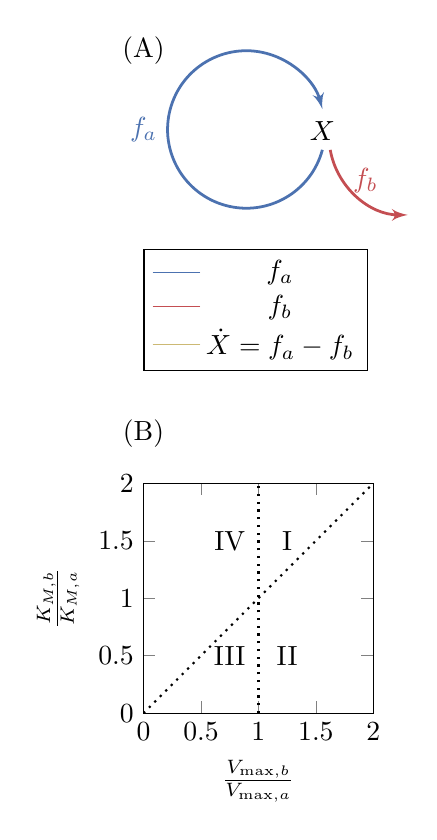
\begin{tikzpicture}[>=latex',node distance = 2cm]
            \node (X) {$X$};
            \draw [->,line width=1pt,autocatacyc] (X.south) arc (345:15:1cm) node [pos=0.5,left] (fa) {$f_a$};
            \draw [->,line width=1pt,branchout] ([xshift=1mm]X.south) arc (190:270:1cm) node [pos=0.3,right] {$f_b$};
            \node [above of=fa,yshift=-1cm] (A) {(A)};
            \begin{customlegend}[legend entries={$f_a$,$f_b$,$\dot{X}=f_a-f_b$},legend style={below=2cm of fa,anchor=west,name=legend1}]
              \addlegendimage{autocatacyc,fill=black!50!red,sharp plot}
              \addlegendimage{branchout,fill=black!50!red,sharp plot}
              \addlegendimage{sumcolor,fill=black!50!red,sharp plot}
            \end{customlegend}
            \begin{axis}[name=phase,xmin=0,ymin=0,xmax=2,ymax=2,xlabel={$\frac{V_{\max,b}}{V_{\max,a}}$},ylabel={$\frac{K_{M,b}}{K_{M,a}}$},samples=6,at=(legend1.south west),anchor=above north west,width=4.5cm,height=4.5cm,yshift=-1.2cm]
            \addplot[domain=0:4,dotted,black,thick] {x};
            \addplot[dotted,black,thick] coordinates {(1,0) (1,2)};
            \node (one) at (axis cs:1.25,1.5) {I};
            \node (two) at (axis cs:1.25,0.5) {II};
            \node (three) at (axis cs:0.75,0.5) {III};
            \node (four) at (axis cs:0.75,1.5) {IV};
          \end{axis}
          \node [at=(legend1.south west),yshift=-0.8cm] (B) {(B)};
         \end{tikzpicture}}%
       \end{minipage}
       \hfill
       \begin{minipage}[c]{.65\linewidth}
        {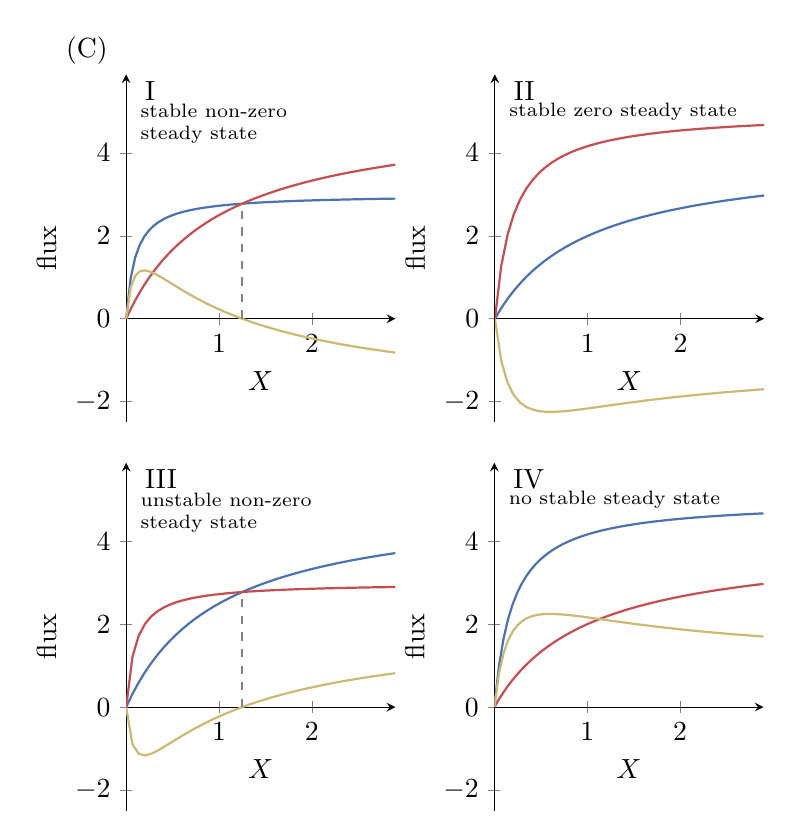
\begin{tikzpicture}
            \begin{axis}[name=plot1,axis x line=middle,axis y line=left,xlabel near ticks,ylabel near ticks,xmin=0,ymin=-2.5,xmax=2.9,ymax=5.9,xlabel={$X$},ylabel={flux},samples=60,width=5cm,height=6cm,clip=false]
            \addplot[domain=0:2.9,autocatacyc,thick] {3*x/(0.1+x)};
            \addplot[domain=0:2.9,branchout,thick] {5*x/(1+x)};
            \addplot[domain=0:2.9,sumcolor,thick] {3*x/(0.1+x)-5*x/(1+x)};
            \addplot[dashed,gray,thick] coordinates {(1.25,0) (1.25,2.77)};
            \node[right] (one) at (axis cs:0.1,5.5) {I};
            \node[right,align=left] (onetext) at (axis cs:0.05,4.7) {\scriptsize stable non-zero\\[-0.4em]\scriptsize steady state};
          \end{axis}
          \node [at=(plot1.north west),xshift=-0.5cm,yshift=0.3cm] (C) {(C)};

          \begin{axis}[name=plot2,axis x line=middle,axis y line=left,xlabel near ticks,ylabel near ticks,xmin=0,ymin=-2.5,xmax=2.9,ymax=5.9,xlabel={$X$},ylabel={flux},samples=60,at=(plot1.right of south east),anchor=left of south west,width=5cm,height=6cm]
            \addplot[domain=0:4,autocatacyc,thick] {4*x/(1+x)};
            \addplot[domain=0:4,branchout,thick] {5*x/(0.2+x)};
            \addplot[domain=0:4,sumcolor,thick] {4*x/(1+x)-5*x/(0.2+x)};
            \node[right] (two) at (axis cs:0.1,5.5) {II};
            \node[right,align=left] (twotext) at (axis cs:0.05,5) {\scriptsize stable zero steady state};
          \end{axis}

          \begin{axis}[name=plot3,axis x line=middle,axis y line=left,xlabel near ticks,ylabel near ticks,xmin=0,ymin=-2.5,xmax=2.9,ymax=5.9,xlabel={$X$},ylabel={flux},samples=60,at=(plot1.below south west),anchor=above north west,width=5cm,height=6cm,yshift=-0.5cm]
            \addplot[domain=0:4,autocatacyc,thick] {5*x/(1+x)};
            \addplot[domain=0:4,branchout,thick] {3*x/(0.1+x)};
            \addplot[domain=0:4,sumcolor,thick] {5*x/(1+x)-3*x/(0.1+x)};
            \addplot[dashed,gray,thick] coordinates {(1.25,0) (1.25,2.77)};
            \node[right] (three) at (axis cs:0.1,5.5) {III};
            \node[right,align=left] (threetext) at (axis cs:0.05,4.7) {\scriptsize unstable non-zero\\[-0.4em]\scriptsize steady state};
          \end{axis}

          \begin{axis}[name=plot4,axis x line=middle,axis y line=left,xlabel near ticks,ylabel near ticks,xmin=0,ymin=-2.5,xmax=2.9,ymax=5.9,xlabel={$X$},ylabel={flux},samples=60,at=(plot3.right of south east),anchor=left of south west,width=5cm,height=6cm]
            \addplot[domain=0:2.9,autocatacyc,thick] {5*x/(0.2+x)};
            \addplot[domain=0:2.9,branchout,thick] {4*x/(1+x)};
            \addplot[domain=0:2.9,sumcolor,thick] {5*x/(0.2+x)-4*x/(1+x)};
            \node[right] (four) at (axis cs:0.1,5.5) {IV};
            \node[right,align=left] (fourtext) at (axis cs:0.05,5) {\scriptsize  no stable steady state};
         \end{axis}
        \end{tikzpicture}}
       \end{minipage}
      \caption{\label{fig:simplecycle}
        (A) A simple autocatalytic cycle induces two fluxes, $f_a$ and $f_b$ as a function of the concentration of $X$.
        These fluxes follow simple Michaelis Menten kinetics.
        A steady state occurs when $f_a=f_b$, implying that $\dot{X}=0$.
        The cycle always has a steady state at $X=0$.
        The slope of each reaction at $X=0$ is $V_{\max}/K_m$.
        A steady state is stable if at the steady state point $\frac{d\dot{X}}{dX}<0$.
        (B) Each set of kinetic parameters, $V_{\max,a},V_{\max,b},K_{M,a},K_{M,b}$ results in one of four cases (C): 
       (I) there is a stable positive steady state and zero is an unstable steady state; 
       (II) zero is the only non-negative steady state, and it is stable;
       (III) zero is a stable steady state and there is a positive, non-stable steady state; 
       (IV) zero is the only non-negative steady state and it is unstable.}
    \end{figure}

    We characterize the metabolic state of this system by the concentration of the metabolite $X$.
    We note that knowing the concentration of $X$ suffices in order to calculate the fluxes originating from it, $f_a$ and $f_b$, thus fully defining the state of the system.
    A steady state of the system is defined as a concentration, $X^*$, which induces fluxes that keep the concentration steady, such that the total in-flux to $X$ is exactly equal to the total out-flux from it.
    In our example, the outgoing flux from $X$ is $f_a+f_b$ and the incoming flux to $X$ is $2f_a$, so at steady state it holds that:
    \begin{equation}
      \label{eq:xdyna}
      \dot X = \frac{dX}{dt} = 2f_a - (f_a + f_b) = 0
    \end{equation}

    Expanding this condition we get:
    \begin{equation*}
      \dot X = 0 \Rightarrow f_a = f_b \Rightarrow \frac{V_{\max,a}X}{K_{M,a}+X}=\frac{V_{\max,b}X}{K_{M,b}+X}
    \end{equation*}
    which is satisfied either if $X=0$ or if:
    \begin{equation}
      \label{eq:xstst}
      X=\frac{V_{\max,b}K_{M,a}-V_{\max,a}K_{M,b}}{V_{\max,a}-V_{\max,b}}
    \end{equation}
    As physiologically the concentration of $X$ cannot be negative, we get a constraint on the kinetic parameters for which a positive steady state exists:
    \begin{equation*}
      \frac{V_{\max,b}K_{M,a}-V_{\max,a}K_{M,b}}{V_{\max,a}-V_{\max,b}}>0 \Rightarrow \frac{\frac{V_{\max,b}}{K_{M,b}}-\frac{V_{\max,a}}{K_{M,a}}}{V_{\max,a}-V_{\max,b}}>0
    \end{equation*}
    The constraint states that if $V_{\max,a}>V_{\max,b}$ then it must be that $\frac{V_{\max,b}}{K_{M,b}}>\frac{V_{\max,a}}{K_{M,a}}$ and that if $V_{\max,a}<V_{\max,b}$ then $\frac{V_{\max,b}}{K_{M,b}}<\frac{V_{\max,a}}{K_{M,a}}$.
    As $\frac{V_{\max}}{K_m}$ is the slope of the Michaelis Menten function at $X=0$, the constraint implies that in order for a positive steady state to exist, the reaction with higher maximal flux must have a shallower slope at $X=0$.
    This condition can be intuitively understood, as the reaction with shallower slope at $X=0$ has smaller fluxes for small values of $X$, compared with the other reaction, so unless it has higher fluxes than the other reaction for large values of $X$ (meaning that its maximal flux is higher), the two will not intersect.
    This constraint is graphically illustrated in Figure \ref{fig:simplecycle}B where cases (II) and (IV) have no positive steady states, and cases (I) and (III) have a positive steady state.

    While having a positive concentration steady state is an essential condition to sustain flux, it is not sufficient.
    The positive concentration steady state must also be stable to small perturbations.
    Stability with respect to small perturbations is determined by the response of the system to small deviations from the steady state, $X^*$.
    Mathematically, stability dictates that at $X=X^*$ it holds that $\frac{d\dot X}{dX} <0$, as this  implies that for points with a small deviation from the steady state: $X = X^*+\Delta X$ the net flux $\dot X$ will oppose the direction of the deviation.
    If $\Delta X$ is positive then $\dot X$ will be negative at $X^*+\Delta X$, reducing $X$ back to $X^*$, and if $\Delta X$ is negative, $\dot X$ will be positive, increasing $X$ back to $X^*$.

    For the simple kinetics we chose the stability condition requires that:
    \begin{equation*}
      \frac{d\dot X}{dX}\Big\vert_{X^*} = \frac{V_{\max,a}K_{M,a}}{(K_{M,a}+X^*)^2}-\frac{V_{\max,b}K_{M,b}}{(K_{M,b}+X^*)^2}<0
    \end{equation*}
    Substituting for $X^*=0$ gives that $0$ is a stable steady state point if $\frac{V_{\max,a}}{K_{M,a}}<\frac{V_{\max,b}}{K_{M,b}}$ (corresponding to the area below the diagonal in figure \ref{fig:simplecycle}B, where $\frac{V_{\max,b}}{V_{\max,a}}>\frac{K_{M,b}}{K_{M,a}}$ resulting in cases (II) and (III)) and is unstable otherwise.
    For  the non-zero steady state, $X^*=\frac{V_{\max,b}K_{M,a}-V_{\max,a}K_{M,b}}{V_{\max,a}-V_{\max,b}}$, we get the opposite condition, i.e. that it is stable if $\frac{V_{\max,b}}{V_{\max,a}}<\frac{K_{M,b}}{K_{M,a}}$ and unstable otherwise.

    It is worthwhile noting that the stability criteria can be stated in metabolic control terms \cite{Fell1997-bp} as requiring that the elasticity of the biomass reaction at the positive steady state be greater than the elasticity of the autocatalytic reaction:
    \begin{equation*}
      \frac{df_b}{dX}\Big\vert_{X^*}>\frac{df_a}{dX}\Big\vert_{X^*} \Rightarrow \varepsilon^X_b>\varepsilon^X_a
    \end{equation*}
    
    The complete analysis is summed up in Figure \ref{fig:simplecycle}B.
    Domains (I) and (III) represent cases where a positive steady state point exists.
    The domains below the diagonal represent cases where $X^*=0$ is a stable steady state point, and the other steady state, if it exists is unstable (cases (II) and (III)).
    The domains above the diagonal represent cases where $X^*=0$ is an unstable steady state point, and the other steady state, if it exists is stable (cases (I) and (IV)).

    To conclude, for this simple cycle, we get that in order for a positive-concentration stable steady state to exist, two conditions must be satisfied:
    \begin{equation}
    \label{eq:stabconds}
    \begin{dcases}
      & V_{\max,b}>V_{\max,a} \\
      & \frac{V_{\max,b}}{K_{M,b}}<\frac{V_{\max,a}}{K_{M,a}}
    \end{dcases}
    \end{equation}
    meaning that for a high enough concentration of $X$, the biomass generating flux should be higher than the autocatalytic flux, ensuring stability, and that at zero concentration of $X$, the slope of the autocatalytic reaction is steeper than the slope of the biomass generating reaction, ensuring that the two fluxes will be equal for some positive concentration of $X$.

    Interestingly, these conditions imply that if $K_{M,b}<K_{M,a}$ then no positive stable steady state can be achieved, even when allowing changes to the expression levels of the enzymes catalyzing $f_a$ and $f_b$, which only affect $V_{\max,a}$ and $V_{\max,b}$.
    This indicates that stability of autocatalytic cycles results from inherent kinetic properties of the enzymes involved and cannot always be achieved by modulating expression levels, a conclusion that may be critical in metabolic engineering context.
\section{Extensions of the simple autocatalytic cycle model}
    \subsection{Generalizing for different autocatalytic stoichiometries}
    Our initial analysis considered an autocatalytic reaction with $1:2$ stoichiometry, such that for every substrate molecule consumed, two are produced.
    Real-world autocatalytic cycles may have different stoichiometries.
    For example, the CBB cycle has a stoichiometry of $5:6$ so that for every 5 molecules of 5-carbon sugars that the autocatalytic reaction consumes, 6 5-carbon sugars are produced.
    We can generalize our analysis by defining $\gamma$ such that for every molecule of $X$ that $f_a$ consumes, it produces $1+\gamma$ molecules of $X$, where $\gamma$ may be a fraction.
    This extension implies that equation \eqref{eq:xdyna} becomes:

    \begin{equation*}
      \dot X = \frac{dX}{dt} = (1+\gamma)f_a - (f_a + f_b) = 0 \Rightarrow \gamma f_a = f_b \Rightarrow \frac{\gamma V_{\max,a}X}{K_{M,a}+X}=\frac{V_{\max,b}X}{K_{M,b}+X}
    \end{equation*}

    Therefore, all of the mathematical derivations conducted above can be extended to different stoichiometries by replacing $V_{\max,a}$ with $\gamma V_{\max,a}$.

    The steady states of this system are thus $X=0$ and (from equation \eqref{eq:xstst}):
    \begin{equation*}
      X=\frac{V_{\max,b}K_{M,a}-\gamma V_{\max,a}K_{M,b}}{\gamma V_{\max,a}-V_{\max,b}}
    \end{equation*}

    The stability criteria from equation \eqref{eq:stabconds} become:
    \begin{equation*}
    \begin{dcases}
      & V_{\max,b}>\gamma V_{\max,a} \\
      & \frac{V_{\max,b}}{K_{M,b}}<\frac{\gamma V_{\max,a}}{K_{M,a}}
    \end{dcases}
    \end{equation*}
    So the qualitative conditions and observations from the $1:2$ stoichiometry case remain valid but with a constant factor that changes the quantitative relations according to the relevant stoichiometry.

\subsection{Input flux increases the range of parameters for which a stable steady state solution exists}
    Autocatalytic cycles are not stand-alone constructs, but are rather embedded in a larger metabolic network.
    Specifically, such cycles generally have some fueling reactions with input flux to at least some of their intermediate metabolites.
    For example, the CBB cycle can have input flux of fructose-6-phosphate from the catabolism of starch.

    When adding a constant input flux, $f_i$ to our simple system (Figure \ref{fig:inputcycle}A) the steady state condition changes to include this flux, giving:
    \begin{equation*}
      \dot X = \frac{dX}{dt} = f_i + f_a - f_b = 0
    \end{equation*}
    In this model, at $X=0$, $\dot X=f_i>0$ so the concentration of $X$ increases and there is no steady state at zero.
    If $V_{\max,b}>f_i+V_{\max,a}$ then at a large enough value of $X$, $\dot X$ will be negative, implying that at some value of $X$ between these two extremes, $\dot{X}$ attains the value of zero, such that under this condition a positive stable steady state point exists (Figure \ref{fig:inputcycle} (I)).
    This case therefore differs from the case with no input flux analyzed above, as now a positive stable steady state can always be achieved by modifying only $V_{\max,a}$ and/or $V_{\max,b}$.
    In this setup, cells can therefore tune the expression levels of enzymes to meet the needs of a stable steady state flux.

    In cases where $V_{\max,b}<f_i+V_{\max,a}$ either no steady states exist (Figure \ref{fig:inputcycle} (II)), or two positive steady states exist (Figure \ref{fig:inputcycle} (III)).
    The latter case implies that there exists a positive concentration $X$ that satisfies:
    \begin{equation*}
        \dot X = 0 \Rightarrow f_i + f_a(X) - f_b(X) = 0 \Rightarrow f_i+\frac{V_{\max,a}X}{K_{M,a}+X} = \frac{V_{\max,b}X}{K_{M,b}+X}
    \end{equation*}
  In this case, the lower concentration steady state will be stable.

  To conclude, input fluxes change the steady state(s) of autocatalytic cycles.
  When an input flux is present, an autocatalytic cycle can always achieve a non zero, stable steady state by tuning the expression levels of the enzymes forming the cycle.
    \begin{figure}[h!]
      \centering
      \begin{minipage}[c]{0.8\linewidth}%
        {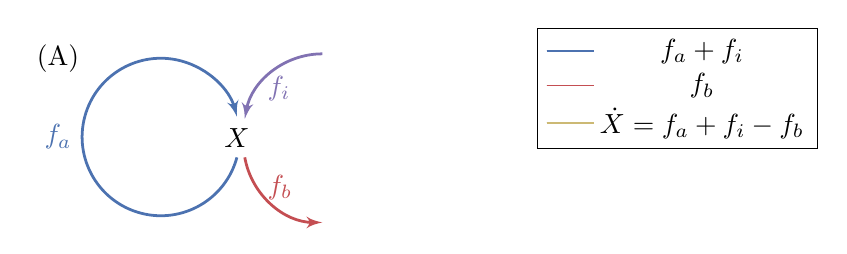
\begin{tikzpicture}[>=latex',node distance = 2cm]
            \node (X) {$X$};
            \draw [->,line width=1pt,autocatacyc] (X.south) arc (345:15:1cm) node [pos=0.5,left] (fa) {$f_a$};
            \draw [->,line width=1pt,branchout] ([xshift=1mm]X.south) arc (190:270:1cm) node [pos=0.3,right] {$f_b$};
            \draw [<-,line width=1pt,magenta] ([xshift=1mm]X.north) arc (170:90:1cm) node [pos=0.3,right] (fi) {$f_i$};
            \node [above of=fa,yshift=-1cm] (A) {(A)};
            \begin{customlegend}[legend entries={$f_a+f_i$,$f_b$,$\dot{X}=f_a+f_i-f_b$},legend style={right=3cm of fi,anchor=west,name=legend1}]
              \addlegendimage{autocatacyc,fill=black!50!red,sharp plot}
              \addlegendimage{branchout,fill=black!50!red,sharp plot}
              \addlegendimage{sumcolor,fill=black!50!red,sharp plot}
            \end{customlegend}
         \end{tikzpicture}}%
       \end{minipage}

       \begin{minipage}[c]{\linewidth}%
        {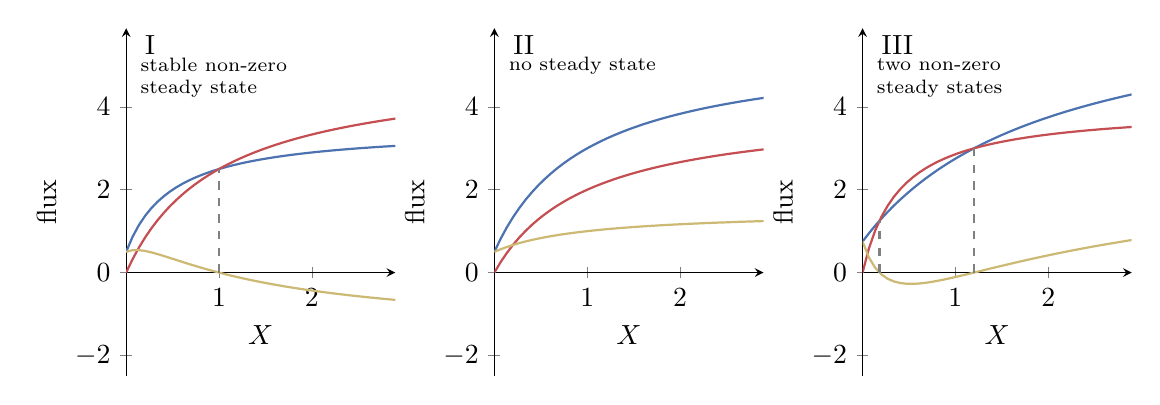
\begin{tikzpicture}
            \begin{axis}[name=plot1,axis x line=middle,axis y line=left,xlabel near ticks,ylabel near ticks,xmin=0,ymin=-2.5,xmax=2.9,ymax=5.9,xlabel={$X$},ylabel={flux},samples=60,width=5cm,height=6cm]
            \addplot[domain=0:4,autocatacyc,thick] {3*x/(0.5+x)+\influx};
            \addplot[domain=0:4,branchout,thick] {5*x/(1+x)};
            \addplot[domain=0:4,sumcolor,thick] {3*x/(0.5+x)-5*x/(1+x)+\influx};
            \addplot[dashed,gray,thick] coordinates {(1,0) (1,2.5)};
            \node[right] (one) at (axis cs:0.1,5.5) {I};
            \node[right,align=left] (onetext) at (axis cs:0.05,4.7) {\scriptsize stable non-zero\\[-0.4em]\scriptsize steady state};
          \end{axis}

          \begin{axis}[name=plot2,axis x line=middle,axis y line=left,xlabel near ticks,ylabel near ticks,xmin=0,ymin=-2.5,xmax=2.9,ymax=5.9,xlabel={$X$},ylabel={flux},samples=60,at=(plot1.right of south east),anchor=left of south west,width=5cm,height=6cm]
            \addplot[domain=0:4,autocatacyc,thick] {5*x/(1+x)+\influx};
            \addplot[domain=0:4,branchout,thick] {4*x/(1+x)};
            \addplot[domain=0:4,sumcolor,thick] {5*x/(1+x)-4*x/(1+x)+\influx};
            \node[right] (two) at (axis cs:0.1,5.5) {II};
            \node[right,align=left] (twotext) at (axis cs:0.05,5) {\scriptsize no steady state};
          \end{axis}

          \begin{axis}[name=plot3,axis x line=middle,axis y line=left,xlabel near ticks,ylabel near ticks,xmin=0,ymin=-2.5,xmax=2.9,ymax=5.9,xlabel={$X$},ylabel={flux},samples=60,at=(plot2.right of south east),anchor=left of south west,width=5cm,height=6cm]
            \addplot[domain=0:4,autocatacyc,thick] {6*x/(2+x)+1.5*\influx};
            \addplot[domain=0:4,branchout,thick] {4*x/(0.4+x)};
            \addplot[domain=0:4,sumcolor,thick] {6*x/(2+x)-4*x/(0.4+x)+1.5*\influx};
            \addplot[dashed,gray,thick] coordinates {(1.2,0) (1.2,3)};
            \addplot[dashed,gray,thick] coordinates {(0.182,0) (0.182,1.25)};
            \node[right] (three) at (axis cs:0.1,5.5) {III};
            \node[right,align=left] (threetext) at (axis cs:0.05,4.7) {\scriptsize two non-zero\\[-0.4em]\scriptsize steady states};
          \end{axis}
        \end{tikzpicture}}
       \end{minipage}
      \caption{\label{fig:inputcycle}
        (A) A simple autocatalytic cycle with a fixed input flux, $f_i$.
        A steady state occurs when $f_a+f_i=f_b$.
        If $V_{\max,b}>V_{\max,a}+f_i$ then there is always a single stable steady state (I).
        If $V_{\max,b}<V_{\max,a}+f_i$ then there can either be no steady states (II), or two steady states where the smaller one is stable (III).
      }
    \end{figure}
    \subsection{Stability analysis for multiple-reaction cycles}
    It is useful to extend the simple criteria we derived to more complex autocatalytic cycles.
    The most straightforward extension is for cycles with more than one intermediate metabolite.
    We start by writing the relevant equations for the two-metabolite autocatalytic cycle depicted in figure \ref{fig:multiple}A.
    In this system there are two intermediate metabolites, $X_1$ and $X_2$, two reactions that form the cycle, $f_{a_1}$ and $f_{a_2}$, and two biomass generating reactions, $f_{b_1}$ and $f_{b_2}$.
    We arbitrarily assume that the autocatalytic reaction is $f_{a_1}$ and that the autocatalysis is in a $1:2$ ratio.
    Given that a steady state of the system exists for some value $X_1^*,X_2^*$ we can evaluate the expression for stability.
    In multi-variable systems, stability dictates that the real part of the eigenvalues of the Jacobian matrix must all be negative for a steady state to be stable.
    We define $\alpha_i=\frac{\partial f_{a_i}}{\partial X_i}$ and $\beta_i=\frac{\partial f_{b_i}}{\partial X_i}$ for $i=1,2$ and get that:
    \begin{equation*}
        J=
        \begin{pmatrix}
            -(\alpha_1+\beta_1) & \alpha_2 \\
            2\alpha_1 & -(\alpha_2+\beta_2)
        \end{pmatrix}
    \end{equation*}
    Solving for the characteristic polynomial gives:
    \begin{align}
        0 & =(\lambda+\alpha_1+\beta_1)(\lambda+\alpha_2+\beta_2)-2\alpha_1\alpha_2 \\
        & = \lambda^2+(\alpha_1+\beta_1+\alpha_2+\beta_2)\lambda+(\alpha_1+\beta_1)(\alpha_2+\beta_2)-2\alpha_1\alpha_2
    \end{align}
    which has two negative roots when:
    \begin{equation}
        (\alpha_1+\beta_1)(\alpha_2+\beta_2)-2\alpha_1\alpha_2>0
    \end{equation}
    The condition is strongly met if $\beta_1\geq \alpha_1$ and $\beta_2\geq\alpha_2$.
    
    The two-metabolites cycle case can be easily extended for a larger number of intermediate metabolites and reactions giving a general characteristic polynomial of:
    \begin{equation}
        0=\prod_{i=1}^n(\lambda+\alpha_i+\beta_i)-2\prod_{i=1}^n\alpha_i
    \end{equation}
    Again, in cases were for all $i$ it holds that $\beta_i\geq\alpha_i$, the eigenvalues will all have negative real values.
    
    To conclude, for the straightforward extension of the simple model to multiple reactions with a single autocatalytic reaction, a sufficient condition for a steady state point to be stable is that at the steady state point the elasticity of each biomass reaction is larger than or equal to the elasticity of the equivalent autocatalytic reaction.
\begin{figure}[h!]
  \centering
    {
        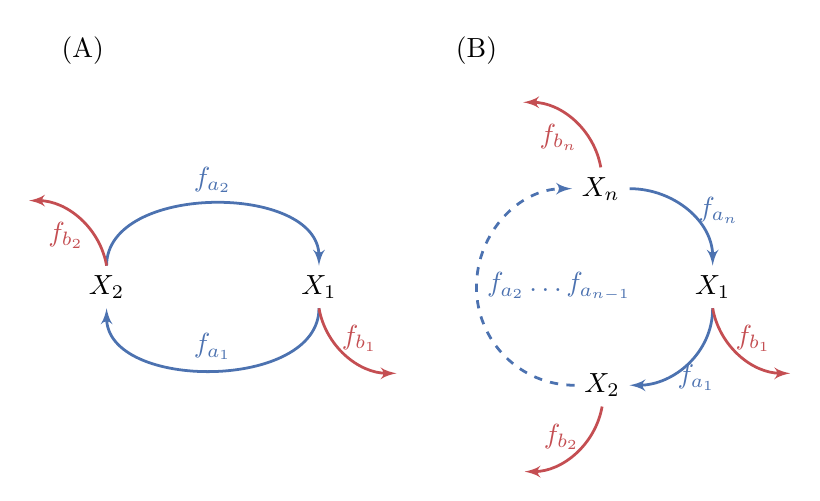
\begin{tikzpicture}[>=latex']
            \begin{scope}[shift={(-5cm,0cm)},node distance = 2cm]
                \node (X1) {$X_1$};
                \node[left=of X1]  (X2) {$X_2$};
                \draw [->,line width=1pt,autocatacyc] (X1.south) [out=-90,in=-90] to  node [pos=0.5,above] (fa1) {$f_{a_1}$} (X2.south);
                \draw [->,line width=1pt,autocatacyc] (X2.north) [out=90,in=90] to  node [pos=0.5,above] (fa2) {$f_{a_2}$} (X1.north);
                \draw [->,line width=1pt,branchout] (X1.south) arc (190:270:1cm) node [pos=0.3,right] {$f_{b_1}$};
                \draw [->,line width=1pt,branchout] (X2.north) arc (10:90:1cm) node [pos=0.3,left] {$f_{b_2}$};
            \end{scope}
            \begin{scope}[shift={(0cm,0cm)},node distance = 1cm]
                \node (X1) {$X_1$};
                \node[below left=of X1]  (X2) {$X_2$};
                \node[above left=of X1]  (Xn) {$X_n$};
                \draw [->,line width=1pt,autocatacyc] (X1.south) [out=-90,in=0] to  node [pos=0.7,right] (fa1) {$f_{a_1}$} (X2.east);
                \draw [->,line width=1pt,autocatacyc] (Xn.east) [out=0,in=90] to  node [pos=0.5,right] (fan) {$f_{a_n}$} (X1.north);
                \draw [->,line width=1pt,branchout] (X1.south) arc (190:270:1cm) node [pos=0.3,right] {$f_{b_1}$};
                \draw [->,line width=1pt,branchout] (X2.south) arc (-10:-90:1cm) node [pos=0.3,left] {$f_{b_2}$};
                \draw [->,line width=1pt,branchout] (Xn.north) arc (10:90:1cm) node [pos=0.3,left] {$f_{b_n}$};
                \draw [->,line width=1pt,autocatacyc,dashed] (X2.west) [out=180,in=-90] to ($(X1)+(-3,0)$) node [right] (fmid) {$f_{a_2}\dots f_{a_{n-1}}$} to [out=90,in=180] (Xn.west);
            \end{scope}
            \node [shift={(-8cm,3cm)}] (A) {(A)};
            \node [right of=A,xshift=4cm] (B) {(B)};
         \end{tikzpicture}
     }
     \caption{Multiple-reaction autocatalytic cycles. (A) A two reaction system. (B) A generic $n$-reaction system. A sufficient condition for the stability of a steady state point in such systems is that the elasticity of each biomass generating reaction is larger than or equal to the elasticity of the equivalent autocatalytic reaction at the steady state concentration.}
     \label{fig:multiple}
\end{figure}
    \subsection{Using different kinetics equations}
    Although we utilized the widely-used irreversible Michaelis-Menten kinetics equation to model enzyme kinetics, our results can be extended to different kinetic equations.
    Generally, two conditions must be met for a stable flux through an autocatalytic cycle to exist: (A) there should be a positive concentration of the intermediate metabolites for which the outgoing fluxes balance the autocatalytic fluxes, resulting in a steady state of fluxes, and, (B) at the steady state point the combined elasticities of the outgoing reactions should be higher, compared with the elasticities of the autocatalytic reactions, to enforce stability in the presence of small perturbations.
    Therefore, these two conditions should be explicitly evaluated for every case with different kinetic equations and autocatalytic cycles topologies to assert whether it can carry stable fluxes or not.

    Two guideline observations can be extracted, regardless of the exact kinetic behavior of the relevant enzymes, though:
    \begin{enumerate}
        \item If a positive flux steady state exists, and the branching reactions have higher $V_{\max}$ values than the autocatalytic reactions, then a positive stable flux steady state is attainable (though it may not necessarily be the same steady state).
        This claim can be deduced as follows:
        If the given steady state is stable, then the claim is obviously correct.
        Otherwise, the given steady state is unstable, so for concentrations slightly above the steady state concentrations, the autocatalytic reactions will drive the intermediate metabolites concentrations to even higher values.
        However, for large enough concentrations of intermediate metabolites the branching reactions will carry higher flux than the autocatalytic reactions, as their $V_{\max}$ values are higher, driving the concentrations of intermediate metabolites down.
        There must therefore be some threshold concentration value below which the autocatalytic reactions carry higher flux, and above which the branching reactions carry higher flux, making this threshold concentration point a stable steady state.
    \item For concentration domains at which the kinetic function of an enzyme is concave, the elasticity of the reaction is anti correlated with the level of saturation of the reaction (where the level of saturation of a reaction is defined as the ratio between the flux through the reaction and the maximal flux it can carry, $V_{\max}$), meaning that the more saturated the reaction is, the lower is its elasticity and vice versa.
          This mathematical property of concave, monotonically increasing, bounded functions clearly follows from the observation that the first derivative of a concave function is a decreasing function, whereas the value of the function, by definition, is an increasing function. 
          As the function is bounded, its saturation is also an increasing function, resulting in an anti correlation between the saturation level and the derivative.
    \end{enumerate}

    These guidelines give a basis for evaluating the stability of operational autocatalytic cycles given fluxomics and proteomics data as is demonstrated below.

    While these guidelines offer sufficient conditions for stability, they are not necessary, meaning a stable steady state can be achieved even in cases where these conditions are not met, or, for example, in cases where the kinetic equations follow a hill function with a coefficient that is larger than 1, making them convex for at least some domain of positive substrate concentrations.
    However, a reasonable and non trivial conclusion from this analysis is that the branching reactions out of a cycle, having a large elasticity at the steady state concentration, cannot be saturated at that point, meaning the enzymes driving the flux out of the cycle and through these reactions are under-utilized resulting in an inherent inefficiency.
    In physiological context this effect is expected to be even higher as the expression pattern of the enzymes must ensure stable fluxes even under expression noise that may alter the amount of both the autocatalytic and the branching reactions enzymes, requiring a large 'buffer zone' to be maintained between the maximal capacity of the branching reactions enzymes versus that of the autocatalytic reactions enzymes.

    \section{Testing the predictions of the analysis on functioning autocatalytic cycles}
    To evaluate the validity of our analysis of autocatalytic cycles we searched for growth conditions under which the autocatalytic cycles we identified in central carbon metabolism carry substantial flux in vivo.
    We used recent in-vivo flux measurements from \cite{Gerosa2015-oq}.

    According to the measurements, two classes of autocatalytic cycles carry substantial flux under at least one of the growth conditions used in \cite{Gerosa2015-oq}:
    the glyoxylate cycle carries significant flux at growth in galactose and acetate;
    PTS using cycles carry significant fluxes at growth in glucose and fructose.

    The PP cycle variants do not carry flux in any of the measured conditions, which is expected given the non-standard metabolites most of their variants assimilate.
    The only physiologically reasonable configuration under which a PP autocatalytic cycle would carry flux is in growth under ribose while missing the rpi reaction, a condition for which no fluxomics measurements are currently available.

    The reverse FBA with ED pathway cycle did not carry flux in any of the measured conditions either.
    Although glycerol could have been a potential carbon source to use this pathway, the metabolic network allows for a more energy efficient growth by using the tpi reaction, following the common lower glycolysis reactions from GAP to pyruvate, avoiding the need to use the less energy efficient ED pathway.

    As noted above, two guidelines for evaluating stability can be explored at major branch points out of a functioning autocatalytic cycle: (A) the maximal flux of the branching reaction, $V_{\max,b}$ should be higher than the maximal flux of the corresponding autocatalytic reaction, $V_{\max,a}$, and, (B) the saturation of the branching reaction should be higher than the saturation of the corresponding autocatalytic reaction.
    We stress again that these conditions are sufficient, but not necessary, for the autocatalytic cycle to be at a stable steady state point.

    To estimate the maximal capacity of a reaction, $V_{\max}$ we followed the procedure described in \cite{Davidi2016-ga}.
    Briefly, for each reaction, under every condition we divided the flux the reaction carries (obtained from \cite{Gerosa2015-oq}) by the amount of the corresponding enzyme expressed under that condition.
    We used data from \cite{Schmidt2015} to obtain the enzyme expression level.
    We thus got a flux per enzyme estimate for the given reaction under each of the conditions.
    We defined the enzyme maximal capacity as the maximum flux per unit enzyme it carries across all reactions.
    Multiplying the enzyme maximal capacity by the enzyme amount at each condition therefore results in an estimate of the maximal possible flux through the given reaction under the relevant condition.


    We used the data from \cite{Gerosa2015-oq} to identify the major branching points in each functioning cycle and the flux distributions in them under each of the relevant conditions.
    The results are presented in figure \ref{fig:branch}.
    The results show that for every functioning autocatalytic cycle, in at least one branching point the biomass generating reaction has a larger maximal flux capacity, and is considerably less saturated than the respective autocatalytic reaction.
    Moreover, out of 9 branching points analyzed, in 6 branching points the branching reactions were significantly less saturated than the autocatalytic reactions, in 2 branching points the saturation levels were similar, and only in one branching point the auto catalytic reaction was less saturated than the branching reaction.

    The branch point that does not agree with our prediction is the branch point in fructose-1,6-bisphosphate at growth with fructose as the carbon source.
    The disagreement arises as a large flux is assigned to the fbp reaction, whereas the corresponding enzyme is not highly expressed.
    This disagreement may be the result of negleting transport of fructose as fructose-6-phosphate, and not fructose-1,6-bisphosphate, which is known to occur in the concentration at which the measurements were made \cite{Kornberg1990-ft}, and which was neglected in \cite{Gerosa2015-oq}.
    Assuming $20\%$ of transported fructose is converted directly to f6p suffices in order to resolve the disagreement, resulting in equal saturation levels for the autocatalytic reaction and the branching reaction.

    The lower saturation values of biomass generating reactions demonstrate that the expressed enzymes have enough capacity to prevent the autocatalytic cycle from increasing the concentration of intermediate metabolites infinitely.
    Moreover, the lower saturation values of the biomass generating reactions suggest that at the steady state point their elasticities are higher, ensuring stable operation of the cycle.

    Another demonstration of the autocatalytic mechanism being at play is in the CBB cycle, which is not a part of the metabolic network of wild type \emph{E.coli}, and for which no flux measurements are available.
    This cycle has been recently introduced synthetically into \emph{E.coli} and was shown to carry flux in it, given further metabolic engineering of central carbon metabolism \cite{Antonovski2016} (cite Antonovsky).
    A key evolutionary event enabling the functioning of the CBB cycle, was a mutation affecting the kinetic properties of the main branching reaction out of the CBB pathway, PRS, reducing its affinity to its substrate, ribose-5p.

    To conclude, while thorough knowledge of the kinetic properties, concentrations and fluxes under various growth conditions is sparse, existing data supports predictions made by our model, given the requirement for stable steady state operation of autocatalytic cycles.
    The model can therefore be used to shed more light on seemingly wasteful investment in the expression of enzymes the capacity of which is not fully utilized, as well as for highlighting at what metabolic branch points enzymes kinetic efficiency may be constrained due to stability requirements of a corresponding autocatalytic cycle.

\begin{figure}[h!]
\centering
\resizebox{1\linewidth}{!}{
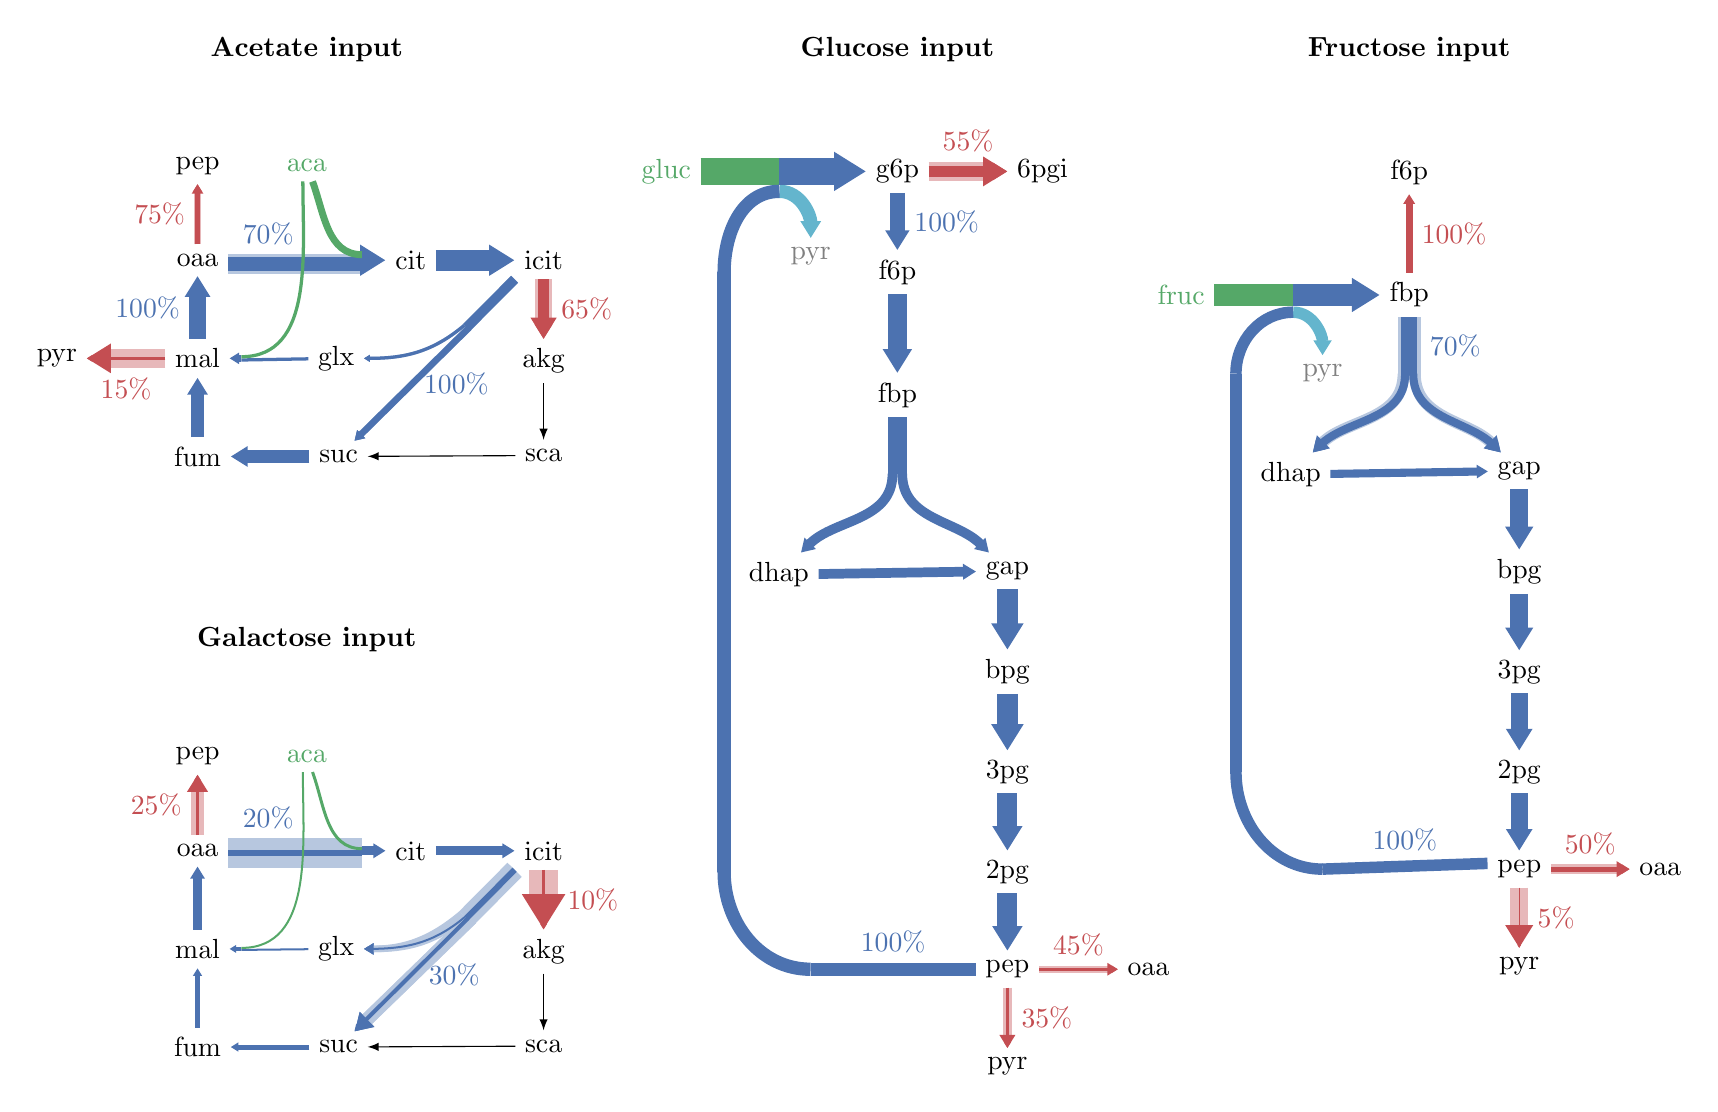
\begin{tikzpicture}
  \tikzset{
    figArrowStyle/.style={arrows={-{Stealth[inset=0pt,scale=#1,angle'=60]}}},
    figArrowStyle/.default=0.25
  }
  \tikzset{
    capArrowStyle/.style={arrows={-{Stealth[inset=0pt,scale=0.25,angle'=60,color=#1]}}},
    capArrowStyle/.default=autocatacyc
    }
  %Galactose
  \begin{scope}[shift={(-6cm,-7.5cm)}]
    \def\galmaxflux{0.5mm}
    \def\galglt{1.52*\galmaxflux}
    \def\galcapvalglt{20}
    \def\galcapglt{\galglt/\galcapvalglt*100}
    \def\galacn{1.52*\galmaxflux*1.5}
    \def\galacea{1.02*\galmaxflux}
    \def\galcapvalacea{30}
    \def\galcapacea{\galacea/\galcapvalacea*100}
    \def\galaceb{1.02*\galmaxflux}
    \def\galsdh{1.26*\galmaxflux}
    \def\galfum{1.26*\galmaxflux}
    \def\galmdh{2.28*\galmaxflux}
    \def\galpck{0.85*\galmaxflux}
    \def\galcapvalpck{25}
    \def\galcappck{\galpck/\galcapvalpck*100}
    \def\galicd{0.5*\galmaxflux}
    \def\galcapvalicd{10}
    \def\galcapicd{\galicd/\galcapvalicd*100}

    \node[] (galactose) {\textbf{Galactose input}};
    \node[metaboliteStyle,inputcol,below=of galactose] (aca) {aca};
    \node[shape=coordinate,below=of aca] (dummyglta) {};
    \node[metaboliteStyle,left=of dummyglta] (oaa) {oaa};
    \node[metaboliteStyle] at (aca -| oaa) (pep) {pep};
    \node[metaboliteStyle,right=of dummyglta] (cit) {cit};
    \node[metaboliteStyle,right=of cit] (icit) {icit};
    \node[metaboliteStyle,below=of icit.center] (akg) {akg};
    \node[metaboliteStyle,below=of akg.center] (sca) {sca};
    \node[metaboliteStyle,below=of oaa.center] (mal) {mal};
    \node[metaboliteStyle,below=of mal.center] (fum) {fum};
    \node[metaboliteStyle,right=of mal] (glx) {glx};
    \node[metaboliteStyle,right=of fum] (suc) {suc};
    \path[] (oaa) -- (cit) node [pos=0.85,shape=coordinate] (midglta) {};
    \draw[line width=\galcapglt,autocatacyc!40] ([yshift=-0.35*\galglt]oaa.east) -- node [above,color=autocatacyc,pos=0.3] {\galcapvalglt\%} ([yshift=-0.35*\galglt]midglta) ;
    \draw[line width=\galglt,autocatacyc] ([yshift=-0.35*\galglt]oaa.east) -- ([yshift=-0.35*\galglt]midglta);
    \draw[figArrowStyle,line width=\galglt*1.5,autocatacyc] (midglta) -- (cit);
    \draw[capArrowStyle=branchout,line width=\galcappck,branchout!40] (oaa) -- node [left,color=branchout] {\galcapvalpck\%}(pep);
    \draw[figArrowStyle,line width=\galpck,branchout] (oaa) -- (pep);
    \draw [inputcol,line width=0.5*\galglt] (aca) [out=-70,in=180] to ([yshift=0.35*\galglt]midglta);
    \draw[figArrowStyle,line width=\galacn,autocatacyc] (cit) -- (icit);
    \path[] (icit.south west) -- (suc) node [pos=0.3,shape=coordinate] (midacea) {};
    \draw[line width=\galcapacea*1.5,autocatacyc!40] (icit.south west) -- (midacea);
    \draw[capArrowStyle,line width=\galcapacea,autocatacyc!40] ([xshift=\galcapacea*0.35]midacea) -- node [right,color=autocatacyc] {\galcapvalacea\%}([xshift=\galcapacea*0.4]suc);
    \draw[capArrowStyle,line width=\galcapacea,autocatacyc!40] ([xshift=\galcapacea*0.38]midacea) -- ([xshift=\galcapacea*0.4]suc);
    \draw[capArrowStyle,line width=\galcapacea*0.5,autocatacyc!40] ([shift={(-\galcapacea*0.35,\galcapacea*0.35)}]midacea) [out=220,in=0] to (glx);
    \draw[capArrowStyle,line width=\galcapacea*0.5,autocatacyc!40] ([shift={(-\galacea*0.35,\galacea*0.35)}]midacea) [out=220,in=0] to (glx);
    \draw[line width=\galacea*1.5,autocatacyc] (icit.south west) -- (midacea);
    \draw[figArrowStyle,line width=\galacea,autocatacyc] ([xshift=\galacea*0.4]midacea) -- ([xshift=\galacea*0.4]suc);
    \draw[figArrowStyle,line width=\galacea*0.5,autocatacyc] ([shift={(-\galacea*0.35,\galacea*0.35)}]midacea) [out=220,in=0] to (glx);
    \draw[capArrowStyle=branchout,line width=\galcapicd*1.5,branchout!40] (icit) -- node [right,color=branchout] {\galcapvalicd\%}(akg);
    \draw[figArrowStyle,line width=\galicd*1.5,branchout] (icit) -- (akg);
    \draw[->] (akg) -- (sca);
    \draw[->] (sca) -- (suc);
    \draw[figArrowStyle,line width=\galsdh,autocatacyc] (suc) -- (fum);
    \draw[figArrowStyle,line width=\galfum,autocatacyc](fum) -- (mal);
    \path[] (glx) -- (mal) node [pos=0.85,shape=coordinate] (midaceb) {};
    \draw[line width=\galaceb*0.5,autocatacyc] ([yshift=-0.25*\galaceb]glx) -- ([yshift=-0.25*\galaceb]midaceb);
    \draw[inputcol,line width=0.5*\galaceb] ([xshift=-0.5mm]aca.south) [out=-90,in=0] to ([yshift=0.25*\galaceb]midaceb);
    \draw[figArrowStyle,line width=\galaceb,autocatacyc] (midaceb) -- (mal);
    \draw[figArrowStyle,line width=\galmdh,autocatacyc] (mal) -- (oaa);
  \end{scope}

  %acetate
  \begin{scope}[shift={(-6cm,0cm)}]
    \def\acemaxflux{0.2mm}
    \def\aceglt{8.83*\acemaxflux}
    \def\acecapvalglt{70}
    \def\acecapglt{\aceglt/\acecapvalglt*100}
    \def\aceacn{8.83*\acemaxflux*1.5}
    \def\aceacea{4.14*\acemaxflux}
    \def\acecapvalacea{100}
    \def\acecapacea{\aceacea}
    \def\aceaceb{4.14*\acemaxflux}
    \def\acesdh{8.4*\acemaxflux}
    \def\acefum{8.4*\acemaxflux}
    \def\acemdh{10.67*\acemaxflux}
    \def\acecapvalmdh{100}
    \def\acemae{1.87*\acemaxflux}
    \def\acecapvalmae{15}
    \def\acecapmae{\acemae/\acecapvalmae*100}
    \def\acepck{3.11*\acemaxflux}
    \def\acecapvalpck{75}
    \def\acecappck{\acepck/\acecapvalpck*100}
    \def\aceicd{4.7*\acemaxflux}
    \def\acecapvalicd{65}
    \def\acecapicd{\aceicd/\acecapvalicd*100}

    \node[] (acetate) {\textbf{Acetate input}};
    \node[metaboliteStyle,inputcol,below=of acetate] (aca) {aca};
    \node[shape=coordinate,below=of aca] (dummyglta) {};
    \node[metaboliteStyle,left=of dummyglta] (oaa) {oaa};
    \node[metaboliteStyle] at (aca -| oaa) (pep) {pep};
    \node[metaboliteStyle,right=of dummyglta] (cit) {cit};
    \node[metaboliteStyle,right=of cit] (icit) {icit};
    \node[metaboliteStyle,below=of icit.center] (akg) {akg};
    \node[metaboliteStyle,below=of akg.center] (sca) {sca};
    \node[metaboliteStyle,below=of oaa.center] (mal) {mal};
    \node[metaboliteStyle,below=of mal.center] (fum) {fum};
    \node[metaboliteStyle,right=of mal] (glx) {glx};
    \node[metaboliteStyle,left=of mal] (pyr) {pyr};
    \node[metaboliteStyle,right=of fum] (suc) {suc};
    \path[] (oaa) -- (cit) node [pos=0.85,shape=coordinate] (midglta) {};
    \draw[line width=\acecapglt,autocatacyc!40] ([yshift=-0.25*\aceglt]oaa.east) --  node [above,color=autocatacyc,pos=0.3] {\acecapvalglt\%}([yshift=-0.25*\aceglt]midglta);
    \draw[line width=\aceglt,autocatacyc] ([yshift=-0.25*\aceglt]oaa.east) -- ([yshift=-0.25*\aceglt]midglta);
    \draw[figArrowStyle,line width=\aceglt*1.5,autocatacyc] (midglta) -- (cit);
    \draw[capArrowStyle=branchout,line width=\acecappck,branchout!40] (oaa) -- node [left,color=branchout] {\acecapvalpck\%}(pep);
    \draw[figArrowStyle,line width=\acepck,branchout] (oaa) -- (pep);
    \draw[capArrowStyle=branchout,line width=\acecapmae,branchout!40] (mal) --  node [below,color=branchout] {\acecapvalmae\%}(pyr);
    \draw[figArrowStyle,line width=\acemae,branchout] (mal) -- (pyr);
    \draw [inputcol,line width=0.5*\aceglt] (aca) [out=-70,in=180] to ([yshift=0.4*\aceglt]midglta);
    \draw[figArrowStyle,line width=\aceacn,autocatacyc] (cit) -- (icit);
    \path[] (icit.south west) -- (suc) node [pos=0.3,shape=coordinate] (midacea) {};
    \draw[line width=\acecapacea*1.5,autocatacyc!40] (icit.south west) -- (midacea);
    \draw[capArrowStyle,line width=\acecapacea,autocatacyc!40] ([xshift=\acecapacea*0.35]midacea) -- node [right,color=autocatacyc] {\acecapvalacea\%}([xshift=\acecapacea*0.4]suc);
    \draw[capArrowStyle,line width=\acecapacea*0.5,autocatacyc!40] ([shift={(-\acecapacea*0.35,\acecapacea*0.35)}]midacea) [out=220,in=0] to (glx);
    \draw[line width=\aceacea*1.5,autocatacyc] (icit.south west) -- (midacea);
    \draw[figArrowStyle,line width=\aceacea,autocatacyc] ([xshift=\aceacea*0.4]midacea) -- ([xshift=\aceacea*0.4]suc);
    \draw[figArrowStyle,line width=\aceacea*0.5,autocatacyc] ([shift={(-\aceacea*0.35,\aceacea*0.35)}]midacea) [out=220,in=0] to (glx);
    \draw[capArrowStyle=branchout,line width=\acecapicd*1.5,branchout!40] (icit) --  node [right,color=branchout] {\acecapvalicd\%}(akg);
    \draw[figArrowStyle,line width=\aceicd*1.5,branchout] (icit) -- (akg);
    \draw[->] (akg) -- (sca);
    \draw[->] (sca) -- (suc);
    \draw[figArrowStyle,line width=\acesdh,autocatacyc] (suc) -- (fum);
    \draw[figArrowStyle,line width=\acefum,autocatacyc](fum) -- (mal);
    \path[] (glx) -- (mal) node [pos=0.85,shape=coordinate] (midaceb) {};
    \draw[line width=\aceaceb*0.5,autocatacyc] ([yshift=-0.25*\aceaceb]glx) -- ([yshift=-0.25*\aceaceb]midaceb);
    \draw[inputcol,line width=0.5*\aceaceb] ([xshift=-0.5mm]aca.south) [out=-90,in=0] to ([yshift=0.25*\aceaceb]midaceb);
    \draw[figArrowStyle,line width=\aceaceb,autocatacyc] (midaceb) -- (mal);
    \draw[figArrowStyle,line width=\acemdh,autocatacyc] (mal) -- node [left,color=autocatacyc] {\acecapvalmdh\%}(oaa);
 
  \end{scope}

  %Glucose
  \begin{scope}[shift={(1.5cm,0cm)}]
    \def\glucmaxflux{0.35mm}
    \def\glucpgi{5.7*\glucmaxflux}
    \def\gluccapvalpgi{100}
    \def\gluccappgi{\glucpgi}
    \def\glucpfk{7.06*\glucmaxflux}
    \def\glucfba{7.06*\glucmaxflux}
    \def\gluctpi{7.06/2*\glucmaxflux}
    \def\glucgap{15.71/2*\glucmaxflux}
    \def\glucpgk{15.71/2*\glucmaxflux}
    \def\glucgpm{14.56/2*\glucmaxflux}
    \def\gluceno{14.56/2*\glucmaxflux}
    \def\glucpyk{2.49/2*\glucmaxflux}
    \def\gluccapvalpyk{35}
    \def\gluccappyk{\glucpyk/\gluccapvalpyk*100}
    \def\glucppc{2.45/2*\glucmaxflux}
    \def\gluccapvalppc{45}
    \def\gluccapppc{\glucppc/\gluccapvalppc*100}
    \def\gluczwf{3.92*\glucmaxflux}
    \def\gluccapvalzwf{55}
    \def\gluccapzwf{\gluczwf/\gluccapvalzwf*100}
    \def\glucpts{9.65*\glucmaxflux}
    \def\gluccapvalpts{100}
    \def\gluccappts{\glucpts}

    \node[] (glucose) {\textbf{Glucose input}};
    \node[metaboliteStyle,below= of glucose] (g6p) {g6p};
    \node[metaboliteStyle,below=of g6p.center] (f6p) {f6p};
    %%% ptstop
    \node[shape=coordinate,left=1.1cm of g6p] (ptsmid) {};
    \node[metaboliteStyle,shift={(-11mm,2mm)},gray] at (f6p) (pyr1) {pyr};
    \node[metaboliteStyle,inputcol,left=of ptsmid] (gluc) {gluc};

    \node[metaboliteStyle,below=of f6p] (fbp) {fbp};
    \node[shape=coordinate,below=of fbp.center](fbamid) {};
    \node[metaboliteStyle,below left=of fbamid.center] (dhap) {dhap};
    \node[metaboliteStyle,below right=of fbamid] (gap) {gap};
    \node[metaboliteStyle,below=of gap.center] (bpg) {bpg};
    \node[metaboliteStyle,below=of bpg.center] (3pg) {3pg};
    \node[metaboliteStyle,below=of 3pg.center] (2pg) {2pg};
    \node[metaboliteStyle,below=of 2pg.center] (pep) {pep};
    \node[metaboliteStyle,right=of pep] (oaa) {oaa};
    \node[metaboliteStyle,below=of pep.center] (pyr) {pyr};
    \node[metaboliteStyle,right=of g6p] (6pgi) {6pgi};
    \draw[figArrowStyle,line width=\glucpgi,autocatacyc] (g6p) -- node [right,color=autocatacyc] {\gluccapvalpgi\%} (f6p);
    \draw[figArrowStyle,line width=\glucpfk,autocatacyc] (f6p.south) -- (fbp.north);
    \draw [line width=\glucfba,autocatacyc] (fbp) [out=-90,in=90] to (fbamid);
    \draw [figArrowStyle,line width=\glucfba/2,autocatacyc] ([xshift=-\glucfba/4]fbamid) [out=-90,in=45] to (dhap);
    \draw [figArrowStyle,line width=\glucfba/2,autocatacyc] ([xshift=\glucfba/4]fbamid) [out=-90,in=135] to (gap);
    \draw [figArrowStyle,line width=\gluctpi,autocatacyc] (dhap) -- (gap);

    \draw[figArrowStyle,line width=\glucgap,autocatacyc] (gap) -- (bpg);
    \draw[figArrowStyle,line width=\glucpgk,autocatacyc] (bpg) -- (3pg);
    \draw[figArrowStyle,line width=\glucgpm,autocatacyc] (3pg) -- (2pg);
    \draw[figArrowStyle,line width=\gluceno,autocatacyc] (2pg) -- (pep);
    \draw[capArrowStyle=branchout,line width=\gluccappyk,branchout!40] (pep) -- node [right,color=branchout] {\gluccapvalpyk\%}(pyr);
    \draw[figArrowStyle,line width=\glucpyk,branchout] (pep) -- (pyr);
    \draw[capArrowStyle=branchout,line width=\gluccapppc,branchout!40] (pep) -- node [above,color=branchout] {\gluccapvalppc\%}(oaa);
    \draw[figArrowStyle,line width=\glucppc,branchout] (pep) -- (oaa);
    \draw[capArrowStyle=branchout,line width=\gluccapzwf,branchout!40] (g6p) -- node [above,color=branchout] {\gluccapvalzwf\%}(6pgi);
    \draw[figArrowStyle,line width=\gluczwf,branchout] (g6p) -- (6pgi);
    %\node[metaboliteStyle,inputcol,shift={(-1.5,-0.8)}] at (pep.center) (gluc) {gluc};
    \node[shape=coordinate,left=2.5cm of pep.center] (pts3) {};
    %\draw[line width=\glucpts/2,autocatacyc] ([yshift=\glucpts/4]pep.west) -- node [above,color=autocatacyc] {\gluccapvalpts\%} ([yshift=\glucpts/4]pts3);
    \draw[line width=\glucpts/2,autocatacyc] (pep.west) -- node [above,color=autocatacyc] {\gluccapvalpts\%} (pts3);
    %\draw[inputcol,line width=\glucpts] ([yshift=-\glucpts/2]gluc) [out=90,in=0] to ([yshift=-\glucpts/2]pts3);
    \draw[inputcol,line width=\glucpts] (gluc) -- (ptsmid);
    \node[shape=coordinate,left=2.5cm of pyr.center] (pts5) {};
    %\draw[line width=\glucpts/2,autocataby] ([yshift=-3*\glucpts/4]pts3) [out=180,in=180] to (pts5);
    %\draw[figArrowStyle,line width=\glucpts/2,autocataby] (pts5) [out=0,in=180] to (pyr);
    \draw[figArrowStyle,line width=\glucpts/2,autocataby] ([yshift=-3/4*\glucpts]ptsmid) [out=0,in=90] to (pyr1);
    \node[shape=coordinate,left=2.2cm of f6p.center] (ptstop) {};
    \node[shape=coordinate] at(ptstop |- 2pg.center) (ptsbottom) {};
    %\draw[line width=\glucpts,autocatacyc] (pts3) [in=-90,out=180] to (ptsbottom);
    \draw[line width=\glucpts/2,autocatacyc] (pts3) [in=-90,out=180] to (ptsbottom);
    %\draw[line width=\glucpts,autocatacyc] (ptsbottom) [in=-90,out=90] to (ptstop);
    \draw[line width=\glucpts/2,autocatacyc] (ptsbottom) -- (ptstop);
    %\draw[figArrowStyle,line width=\glucpts,autocatacyc] (ptstop) [in=180,out=90] to (g6p);
    \draw[line width=\glucpts/2,autocatacyc] (ptstop) [in=180,out=90] to ([yshift=-3/4*\glucpts]ptsmid);
    \draw[figArrowStyle,line width=\glucpts,autocatacyc] (ptsmid) -- (g6p);
  \end{scope}

  %Fructose
  \begin{scope}[shift={(8cm,0cm)}]
    \def\frucmaxflux{0.35mm}
    \def\frucfbp{2.46*\frucmaxflux}
    \def\fruccapvalfbp{100}
    \def\fruccapfbp{\frucfbp}
    \def\frucfba{5.87*\frucmaxflux}
    \def\fruccapvalfba{70}
    \def\fruccapfba{\frucfba/\fruccapvalfba*100}
    \def\fructpi{5.87/2*\frucmaxflux}
    \def\frucgap{13.46/2*\frucmaxflux}
    \def\frucpgk{13.46/2*\frucmaxflux}
    \def\frucgpm{12.6/2*\frucmaxflux}
    \def\fruceno{12.6/2*\frucmaxflux}
    \def\frucpyk{0.67/2*\frucmaxflux}
    \def\fruccapvalpyk{5}
    \def\fruccappyk{\frucpyk/\fruccapvalpyk*100}
    \def\frucppc{3.55/2*\frucmaxflux}
    \def\fruccapvalppc{50}
    \def\fruccapppc{\frucppc/\fruccapvalppc*100}
    \def\frucpts{8.33*\frucmaxflux}
    \def\fruccapvalpts{100}
    \def\fruccappts{\frucpts}


    \node[] (fructose) {\textbf{Fructose input}};
    \node[metaboliteStyle,below=of fructose] (f6p) {f6p};
    \node[metaboliteStyle,below=of f6p] (fbp) {fbp};
    \node[shape=coordinate,below=of fbp.center](fbamid) {};
    %%% ptstop
    \node[shape=coordinate,left=1.1cm of fbp] (ptsmid) {};
    \node[metaboliteStyle,shift={(-11mm,0mm)},gray] at (fbamid) (pyr1) {pyr};
    \node[metaboliteStyle,inputcol,left=of ptsmid] (fruc) {fruc};

    \node[metaboliteStyle,below left=of fbamid.center] (dhap) {dhap};
    \node[metaboliteStyle,below right=of fbamid] (gap) {gap};
    \node[metaboliteStyle,below=of gap.center] (bpg) {bpg};
    \node[metaboliteStyle,below=of bpg.center] (3pg) {3pg};
    \node[metaboliteStyle,below=of 3pg.center] (2pg) {2pg};
    \node[metaboliteStyle,below=of 2pg.center] (pep) {pep};
    \node[metaboliteStyle,right=of pep] (oaa) {oaa};
    \node[metaboliteStyle,below=of pep.center] (pyr) {pyr};
    \draw[figArrowStyle,line width=\frucfbp,branchout] (fbp)-- node [right,color=branchout] {\fruccapvalfbp\%}(f6p) ;
    \draw [line width=\fruccapfba,autocatacyc!40] (fbp) -- node [right,color=autocatacyc] {\fruccapvalfba\%}(fbamid);
    \draw [capArrowStyle,line width=\fruccapfba/2,autocatacyc!40] ([xshift=-\fruccapfba/4]fbamid) [out=-90,in=45] to (dhap);
    \draw [capArrowStyle,line width=\fruccapfba/2,autocatacyc!40] ([xshift=\fruccapfba/4]fbamid) [out=-90,in=135] to (gap);
    \draw [line width=\frucfba,autocatacyc] (fbp) [out=-90,in=90] to (fbamid);
    \draw [figArrowStyle,line width=\frucfba/2,autocatacyc] ([xshift=-\frucfba/4]fbamid) [out=-90,in=45] to (dhap);
    \draw [figArrowStyle,line width=\frucfba/2,autocatacyc] ([xshift=\frucfba/4]fbamid) [out=-90,in=135] to (gap);
    \draw [figArrowStyle,line width=\fructpi,autocatacyc] (dhap) -- (gap);

    \draw[figArrowStyle,line width=\frucgap,autocatacyc] (gap) -- (bpg);
    \draw[figArrowStyle,line width=\frucpgk,autocatacyc] (bpg) -- (3pg);
    \draw[figArrowStyle,line width=\frucgpm,autocatacyc] (3pg) -- (2pg);
    \draw[figArrowStyle,line width=\fruceno,autocatacyc] (2pg) -- (pep);
    \draw[capArrowStyle=branchout,line width=\fruccappyk,branchout!40] (pep) -- node [right,color=branchout] {\fruccapvalpyk\%}(pyr);
    \draw[figArrowStyle,line width=\frucpyk,branchout] (pep) -- (pyr);
    \draw[capArrowStyle=branchout,line width=\fruccapppc,branchout!40] (pep) -- node [above,color=branchout] {\fruccapvalppc\%}(oaa);
    \draw[figArrowStyle,line width=\frucppc,branchout] (pep) -- (oaa);
    \node[shape=coordinate,left=2.5cm of pep.center] (pts3) {};
    %\draw[line width=\frucpts/2,autocatacyc] ([yshift=\frucpts/4]pep.west) -- node [above,color=autocatacyc] {\fruccapvalpts\%}([yshift=\frucpts/4]pts3);
    \draw[line width=\frucpts/2,autocatacyc] ([yshift=\frucpts/4]pep.west) -- node [above,color=autocatacyc] {\fruccapvalpts\%}(pts3);
    \node[shape=coordinate,left=2.5cm of pyr.center] (pts5) {};
    %\draw[line width=\frucpts/2,autocataby] ([yshift=-3*\frucpts/4]pts3) [out=180,in=180] to (pts5);
    %\draw[figArrowStyle,line width=\frucpts/2,autocataby] (pts5) [out=0,in=180] to (pyr);
    \draw[figArrowStyle,line width=\frucpts/2,autocataby] ([yshift=-3/4*\frucpts]ptsmid) [out=0,in=90] to (pyr1);
    \node[shape=coordinate,left=2.2cm of fbamid] (ptstop) {};
    \node[shape=coordinate] at(ptstop |- 2pg.center) (ptsbottom) {};
    \draw[] (pts3) [in=-90,out=180] to (ptsbottom);
    \draw[] (ptsbottom) [in=-90,out=90] to (ptstop);
    %\node[metaboliteStyle,inputcol,shift={(-1.5,-0.8)}] at (pep.center) (fruc) {fruc};
    %\draw[inputcol,line width=\frucpts] ([yshift=-\frucpts/2]fruc) [out=90,in=0] to ([yshift=-\frucpts/2]pts3);
    \draw[inputcol,line width=\frucpts] (fruc) -- (ptsmid);
    \draw[line width=\frucpts/2,autocatacyc] (pts3) [in=-90,out=180] to (ptsbottom);
    \draw[line width=\frucpts/2,autocatacyc] (ptsbottom) -- (ptstop);
    %\draw[figArrowStyle,line width=\frucpts,autocatacyc] (ptstop) [in=180,out=90] to (fbp);
    \draw[line width=\frucpts/2,autocatacyc] (ptstop) [in=180,out=90] to ([yshift=-3/4*\frucpts]ptsmid);
    \draw[figArrowStyle,line width=\frucpts,autocatacyc] (ptsmid) -- (fbp);
  \end{scope}
  \end{tikzpicture}
}
\caption{
  Major branch points and relative enzyme saturation in operating autocatalytic cycles. In all cases there is enough excess capacity in the branching reactions to prevent the cycle from overflowing. Moreover, only in one out of the 8 branch points observed (the branch point at fbp in growth under fructose), an outgoing reaction is significantly more saturated than the autocatalytic reaction.
}
    \label{fig:branch}
\end{figure}


\section{Discussion}
A common concept in synthetic biology is that the successful implementation of novel pathways requires the expression of functional enzymes in the correct amounts in the target organism.
Here we show that in the specific context of the newly introduced enzymes being involved in autocatalytic cycles, such a successful expression may not suffice.
Specifically, changes to some of the kinetic parameters of enzymes at branch points of the cycle may be required in order for the novel pathway to function.

Another aspect of our findings is that while generally, high affinity and catalytic rate are desirable traits for enzymes, in the specific context of autocatalytic cycles, constraints may exist on the relations between these kinetic parameters across different enzymes rendering improvements in only some of them deleterious for the functioning of the cycle.
Moreover, in order for a cycle to be stable, at least some of the enzymes catalyzing reactions out of the cycles may need to be over-expressed, resulting in a seemingly inefficient expression pattern that is required in order to ensure that branching reactions are less saturated than the corresponding autocatalytic reactions.

A recent demonstration of these principles in vivo is the implementation of a functional CBB cycle in \emph{e.coli} by introducing the two genes missing for its functioning \cite{Antonovski2016}.
The successful introduction of the genes did not suffice to make the cycle function, and further directed evolution was needed in order to achieve non-zero flux through the cycle.
A key change in the evolutionary process was the decrease of the affinity of phosphoribosylpyrophosphate synthetase (PRS), one of the enzymes responsible for flux out of the CBB cycle, corresponding to the biomass reaction in our simple model.

Our observation regarding the stabilizing effect of input fluxes into an autocatalytic cycle may provide some means to mitigate the stability issue in synthetic biology metabolic engineering setups, allowing for a pathway to gradually evolve towards sustainable, substantial flux.

More generally, whereas in usual metabolic context a higher flux through a reaction will not decrease the flux into any of its reactants (it may increase this flux if one of the reactions feeding into the reactant is reversible), in setups involving autocatalytic cycles, such negative feedback exists as an inherent structural feature of the system.

While autocatalytic cycles are usually considered a small part of metabolism, with less than a handful of examples, we note that by the definition presented here, such cycles are abundant even in central carbon metabolism.
The examples of autocatalytic cycles we provide, as well as our verified predictions on the economical usage of enzymes catalyzing reactions branching out of such cycles, suggest that the constraints we find on the kinetic parameters of enzymes involved in autocatalytic cycles may confine and shape the kinetic parameters of a broad set of enzymes central to metabolism.

  Finally, while our work focuses on cycles increasing the amount of carbon in the system, we note that autocatalysis can be defined with respect to other quantities such as energy (in the form of high energy phosphate bonds), non-carbon atoms, reducing power, or other moieties.
  Work along these lines is presented in \cite{Reich1981-qd}.
  The mathematical analysis we present here can technically apply for such definitions as well and may thus be used beyond the context presented in this work.
\section{Acknowledgments}
We would like to thank Arren Bar-Even, Katja Tummler, Daniel Segre, Matthias Heinemann, David Fell, Patrick Shih, Wolfram Liebermeister  and \dots for fruitful discussions and valuable insights contributing to this work.
%(Acknowledge tikz/latex/pgf/xcolor/stackexchange community for supporting free software tools)
\bibliography{library}{}
\bibliographystyle{ieeetr}
\end{document}
